\documentclass[journal]{IEEEtran}

%% =========================================================================
%% Knowledge-Base Poisoning of Retrieval-Augmented Generation Under a
%% Compromised Authorized Publisher
%%
%% Regular Paper prepared for IEEE Transactions on Information Forensics and
%% Security. Initial submissions are limited to 13 double-column pages.
%%
%% Compile:  pdflatex MainPaper && bibtex MainPaper && pdflatex MainPaper && pdflatex MainPaper
%%
%% Result tables, figures, and aggregate macros are regenerated from
%% paper-submission/artifacts/; no result number is typed by hand where a
%% generated macro exists.
%% =========================================================================

\usepackage{cite}
\usepackage{amsmath}
\usepackage{amssymb}
\usepackage{graphicx}
\usepackage{booktabs}
\usepackage{array}
\usepackage{tabularx}
\usepackage{changepage}
\usepackage{algorithm}
\usepackage{algpseudocode}
\usepackage{url}
\usepackage[colorlinks=true,citecolor=blue,linkcolor=blue,urlcolor=blue]{hyperref}

%% The generated tables wrap their bodies in adjustwidth with this allowance.
\newlength{\extralength}
\setlength{\extralength}{0pt}

\newcommand{\AdvU}{\mathcal{U}}
\newcommand{\AdvC}{\mathcal{C}}
\newcommand{\prin}{\mathsf{pr}}

%% Result values are generated from the compact, versioned artifact bundle.
% Generated by ragsec.eval.report - do not edit by hand.
\newcommand{\asrStaticSquadnone}{0.95}
\newcommand{\casrStaticSquadnone}{0.96}
\newcommand{\asrAdaptiveSquadnone}{0.81}
\newcommand{\casrAdaptiveSquadnone}{0.83}
\newcommand{\casrFloodingSquadnone}{1.00}
\newcommand{\asrFloodingSquadnone}{1.00}
\newcommand{\asrStaticSquadLOne}{0.10}
\newcommand{\casrStaticSquadLOne}{0.01}
\newcommand{\asrAdaptiveSquadLOne}{0.81}
\newcommand{\casrAdaptiveSquadLOne}{0.83}
\newcommand{\casrFloodingSquadLOne}{0.00}
\newcommand{\asrFloodingSquadLOne}{0.38}
\newcommand{\asrStaticSquadLTwo}{0.11}
\newcommand{\casrStaticSquadLTwo}{0.02}
\newcommand{\asrAdaptiveSquadLTwo}{0.81}
\newcommand{\casrAdaptiveSquadLTwo}{0.83}
\newcommand{\casrFloodingSquadLTwo}{0.04}
\newcommand{\asrFloodingSquadLTwo}{0.42}
\newcommand{\asrStaticSquadLThree}{0.69}
\newcommand{\casrStaticSquadLThree}{0.68}
\newcommand{\asrAdaptiveSquadLThree}{0.84}
\newcommand{\casrAdaptiveSquadLThree}{0.86}
\newcommand{\casrFloodingSquadLThree}{0.99}
\newcommand{\asrFloodingSquadLThree}{1.00}
\newcommand{\asrStaticSquadLFour}{0.95}
\newcommand{\casrStaticSquadLFour}{0.96}
\newcommand{\asrAdaptiveSquadLFour}{0.81}
\newcommand{\casrAdaptiveSquadLFour}{0.83}
\newcommand{\casrFloodingSquadLFour}{1.00}
\newcommand{\asrFloodingSquadLFour}{1.00}
\newcommand{\asrStaticSquadfull}{0.13}
\newcommand{\casrStaticSquadfull}{0.00}
\newcommand{\asrAdaptiveSquadfull}{0.82}
\newcommand{\casrAdaptiveSquadfull}{0.83}
\newcommand{\casrFloodingSquadfull}{0.00}
\newcommand{\asrFloodingSquadfull}{0.49}
\newcommand{\asrStaticSquadfullsigned}{0.13}
\newcommand{\casrStaticSquadfullsigned}{0.00}
\newcommand{\asrAdaptiveSquadfullsigned}{0.00}
\newcommand{\casrAdaptiveSquadfullsigned}{0.00}
\newcommand{\casrFloodingSquadfullsigned}{0.00}
\newcommand{\asrFloodingSquadfullsigned}{0.49}
\newcommand{\cleanAccSquadnone}{0.62}
\newcommand{\cleanAccSquadLOne}{0.62}
\newcommand{\cleanAccSquadLTwo}{0.61}
\newcommand{\cleanAccSquadLThree}{0.52}
\newcommand{\cleanAccSquadLFour}{0.62}
\newcommand{\cleanAccSquadfull}{0.51}
\newcommand{\cleanAccSquadfullsigned}{0.51}
\newcommand{\asrStaticHotpotqanone}{0.96}
\newcommand{\casrStaticHotpotqanone}{0.97}
\newcommand{\asrAdaptiveHotpotqanone}{0.95}
\newcommand{\casrAdaptiveHotpotqanone}{0.97}
\newcommand{\casrFloodingHotpotqanone}{1.00}
\newcommand{\asrFloodingHotpotqanone}{1.00}
\newcommand{\asrStaticHotpotqaLOne}{0.19}
\newcommand{\casrStaticHotpotqaLOne}{0.01}
\newcommand{\asrAdaptiveHotpotqaLOne}{0.95}
\newcommand{\casrAdaptiveHotpotqaLOne}{0.97}
\newcommand{\casrFloodingHotpotqaLOne}{0.00}
\newcommand{\asrFloodingHotpotqaLOne}{0.75}
\newcommand{\asrStaticHotpotqaLTwo}{0.19}
\newcommand{\casrStaticHotpotqaLTwo}{0.00}
\newcommand{\asrAdaptiveHotpotqaLTwo}{0.96}
\newcommand{\casrAdaptiveHotpotqaLTwo}{0.97}
\newcommand{\casrFloodingHotpotqaLTwo}{0.00}
\newcommand{\asrFloodingHotpotqaLTwo}{0.74}
\newcommand{\asrStaticHotpotqaLThree}{0.72}
\newcommand{\casrStaticHotpotqaLThree}{0.71}
\newcommand{\asrAdaptiveHotpotqaLThree}{0.96}
\newcommand{\casrAdaptiveHotpotqaLThree}{0.98}
\newcommand{\casrFloodingHotpotqaLThree}{1.00}
\newcommand{\asrFloodingHotpotqaLThree}{0.99}
\newcommand{\asrStaticHotpotqaLFour}{0.96}
\newcommand{\casrStaticHotpotqaLFour}{0.97}
\newcommand{\asrAdaptiveHotpotqaLFour}{0.95}
\newcommand{\casrAdaptiveHotpotqaLFour}{0.97}
\newcommand{\casrFloodingHotpotqaLFour}{1.00}
\newcommand{\asrFloodingHotpotqaLFour}{1.00}
\newcommand{\asrStaticHotpotqafull}{0.20}
\newcommand{\casrStaticHotpotqafull}{0.01}
\newcommand{\asrAdaptiveHotpotqafull}{0.90}
\newcommand{\casrAdaptiveHotpotqafull}{0.95}
\newcommand{\casrFloodingHotpotqafull}{0.00}
\newcommand{\asrFloodingHotpotqafull}{0.81}
\newcommand{\asrStaticHotpotqafullsigned}{0.20}
\newcommand{\casrStaticHotpotqafullsigned}{0.01}
\newcommand{\asrAdaptiveHotpotqafullsigned}{0.01}
\newcommand{\casrAdaptiveHotpotqafullsigned}{0.01}
\newcommand{\casrFloodingHotpotqafullsigned}{0.00}
\newcommand{\asrFloodingHotpotqafullsigned}{0.81}
\newcommand{\cleanAccHotpotqanone}{0.25}
\newcommand{\cleanAccHotpotqaLOne}{0.25}
\newcommand{\cleanAccHotpotqaLTwo}{0.26}
\newcommand{\cleanAccHotpotqaLThree}{0.19}
\newcommand{\cleanAccHotpotqaLFour}{0.25}
\newcommand{\cleanAccHotpotqafull}{0.19}
\newcommand{\cleanAccHotpotqafullsigned}{0.19}
\newcommand{\asrStaticToynone}{0.87}
\newcommand{\casrStaticToynone}{0.87}
\newcommand{\asrAdaptiveToynone}{0.46}
\newcommand{\casrAdaptiveToynone}{0.46}
\newcommand{\casrFloodingToynone}{0.87}
\newcommand{\asrFloodingToynone}{0.87}
\newcommand{\asrStaticToyLOne}{0.00}
\newcommand{\casrStaticToyLOne}{0.00}
\newcommand{\asrAdaptiveToyLOne}{0.46}
\newcommand{\casrAdaptiveToyLOne}{0.46}
\newcommand{\casrFloodingToyLOne}{0.00}
\newcommand{\asrFloodingToyLOne}{0.00}
\newcommand{\asrStaticToyLTwo}{0.03}
\newcommand{\casrStaticToyLTwo}{0.00}
\newcommand{\asrAdaptiveToyLTwo}{0.52}
\newcommand{\casrAdaptiveToyLTwo}{0.47}
\newcommand{\casrFloodingToyLTwo}{0.00}
\newcommand{\asrFloodingToyLTwo}{0.10}
\newcommand{\asrStaticToyLThree}{0.58}
\newcommand{\casrStaticToyLThree}{0.58}
\newcommand{\asrAdaptiveToyLThree}{1.00}
\newcommand{\casrAdaptiveToyLThree}{1.00}
\newcommand{\casrFloodingToyLThree}{0.87}
\newcommand{\asrFloodingToyLThree}{0.87}
\newcommand{\asrStaticToyLFour}{0.87}
\newcommand{\casrStaticToyLFour}{0.87}
\newcommand{\asrAdaptiveToyLFour}{0.46}
\newcommand{\casrAdaptiveToyLFour}{0.46}
\newcommand{\casrFloodingToyLFour}{0.87}
\newcommand{\asrFloodingToyLFour}{0.87}
\newcommand{\asrStaticToyfull}{0.03}
\newcommand{\casrStaticToyfull}{0.00}
\newcommand{\asrAdaptiveToyfull}{0.94}
\newcommand{\casrAdaptiveToyfull}{0.94}
\newcommand{\casrFloodingToyfull}{0.00}
\newcommand{\asrFloodingToyfull}{0.10}
\newcommand{\asrStaticToyfullsigned}{0.03}
\newcommand{\casrStaticToyfullsigned}{0.00}
\newcommand{\asrAdaptiveToyfullsigned}{0.00}
\newcommand{\casrAdaptiveToyfullsigned}{0.00}
\newcommand{\casrFloodingToyfullsigned}{0.00}
\newcommand{\asrFloodingToyfullsigned}{0.10}
\newcommand{\cleanAccToynone}{1.00}
\newcommand{\cleanAccToyLOne}{1.00}
\newcommand{\cleanAccToyLTwo}{0.90}
\newcommand{\cleanAccToyLThree}{1.00}
\newcommand{\cleanAccToyLFour}{1.00}
\newcommand{\cleanAccToyfull}{0.90}
\newcommand{\cleanAccToyfullsigned}{0.90}
\newcommand{\evasionFullNone}{0.82}
\newcommand{\evasionFullsignedNone}{0.00}
\newcommand{\evasionFullParaphrase}{0.00}
\newcommand{\evasionFullsignedParaphrase}{0.00}
\newcommand{\evasionFullNodirectives}{0.00}
\newcommand{\evasionFullsignedNodirectives}{0.00}
\newcommand{\evasionFullNaturalpadding}{0.82}
\newcommand{\evasionFullsignedNaturalpadding}{0.00}
\newcommand{\evasionFullDilutesimilarity}{0.82}
\newcommand{\evasionFullsignedDilutesimilarity}{0.00}
\newcommand{\evasionFullSpoofsource}{0.00}
\newcommand{\evasionFullsignedSpoofsource}{0.00}
\newcommand{\evasionFullDiversify}{0.82}
\newcommand{\evasionFullsignedDiversify}{0.00}
\newcommand{\provQuotaAdaptiveHotpot}{0.95}
\newcommand{\provSignedAdaptiveHotpot}{0.00}
\newcommand{\provOpenStatic}{0.99}
\newcommand{\provOpenAdaptive}{0.81}
\newcommand{\provTrustonlyStatic}{0.01}
\newcommand{\provTrustonlyAdaptive}{0.81}
\newcommand{\provAllowlistStatic}{0.01}
\newcommand{\provAllowlistAdaptive}{0.81}
\newcommand{\provQuotaStatic}{0.01}
\newcommand{\provQuotaAdaptive}{0.14}
\newcommand{\provSignedStatic}{0.01}
\newcommand{\provSignedAdaptive}{0.01}
\newcommand{\aurocAdaptiveSquad}{0.47}
\newcommand{\aurocStaticMinSquad}{0.99}
\newcommand{\aurocAdaptiveHotpotqa}{0.65}
\newcommand{\aurocStaticMinHotpotqa}{0.97}
\newcommand{\aurocAdaptiveToy}{0.31}
\newcommand{\aurocStaticMinToy}{0.99}
\newcommand{\auprcAdaptiveSquad}{0.56}
\newcommand{\auprcStaticMinSquad}{0.99}
\newcommand{\auprcAdaptiveHotpotqa}{0.47}
\newcommand{\auprcStaticMinHotpotqa}{0.93}
\newcommand{\auprcAdaptiveToy}{0.65}
\newcommand{\auprcStaticMinToy}{0.99}
\newcommand{\tprAdaptiveSquad}{0.00}
\newcommand{\tprAdaptiveHotpotqa}{0.02}
\newcommand{\tprAdaptiveToy}{0.00}
\newcommand{\tauDefault}{1.0}
\newcommand{\tauDefaultTprAdaptive}{0.00}
\newcommand{\tauDefaultAsrAdaptive}{0.83}
\newcommand{\tauDefaultCleanAcc}{0.61}
\newcommand{\tauDefaultFpr}{0.01}
\newcommand{\tauModerate}{0.7}
\newcommand{\tauModerateTprAdaptive}{0.20}
\newcommand{\tauModerateAsrAdaptive}{0.49}
\newcommand{\tauModerateCleanAcc}{0.25}
\newcommand{\tauModerateFpr}{0.09}
\newcommand{\tauAggressive}{0.5}
\newcommand{\tauAggressiveTprAdaptive}{0.76}
\newcommand{\tauAggressiveAsrAdaptive}{0.07}
\newcommand{\tauAggressiveCleanAcc}{0.06}
\newcommand{\tauAggressiveFpr}{0.56}
\newcommand{\budgetAdaptiveNoneSquadBOne}{0.82}
\newcommand{\budgetAdaptiveNoneSquadBTwo}{0.82}
\newcommand{\budgetAdaptiveNoneSquadBThree}{0.83}
\newcommand{\budgetAdaptiveNoneSquadBFive}{0.84}
\newcommand{\budgetAdaptiveNoneSquadBTen}{0.85}
\newcommand{\budgetAdaptiveNoneSquadBTwenty}{0.85}
\newcommand{\budgetAdaptiveFullSquadBOne}{0.69}
\newcommand{\budgetAdaptiveFullSquadBTwo}{0.83}
\newcommand{\budgetAdaptiveFullSquadBThree}{0.83}
\newcommand{\budgetAdaptiveFullSquadBFive}{0.84}
\newcommand{\budgetAdaptiveFullSquadBTen}{0.86}
\newcommand{\budgetAdaptiveFullSquadBTwenty}{0.88}
\newcommand{\budgetAdaptiveSignedSquadBOne}{0.00}
\newcommand{\budgetAdaptiveSignedSquadBTwo}{0.00}
\newcommand{\budgetAdaptiveSignedSquadBThree}{0.00}
\newcommand{\budgetAdaptiveSignedSquadBFive}{0.00}
\newcommand{\budgetAdaptiveSignedSquadBTen}{0.00}
\newcommand{\budgetAdaptiveSignedSquadBTwenty}{0.00}
\newcommand{\budgetStaticNoneSquadBOne}{0.99}
\newcommand{\budgetStaticNoneSquadBTwo}{0.99}
\newcommand{\budgetStaticNoneSquadBThree}{0.99}
\newcommand{\budgetStaticNoneSquadBFive}{0.99}
\newcommand{\budgetStaticNoneSquadBTen}{1.00}
\newcommand{\budgetStaticNoneSquadBTwenty}{1.00}
\newcommand{\budgetStaticFullSquadBOne}{0.00}
\newcommand{\budgetStaticFullSquadBTwo}{0.00}
\newcommand{\budgetStaticFullSquadBThree}{0.00}
\newcommand{\budgetStaticFullSquadBFive}{0.00}
\newcommand{\budgetStaticFullSquadBTen}{0.00}
\newcommand{\budgetStaticFullSquadBTwenty}{0.00}
\newcommand{\budgetStaticSignedSquadBOne}{0.00}
\newcommand{\budgetStaticSignedSquadBTwo}{0.00}
\newcommand{\budgetStaticSignedSquadBThree}{0.00}
\newcommand{\budgetStaticSignedSquadBFive}{0.00}
\newcommand{\budgetStaticSignedSquadBTen}{0.00}
\newcommand{\budgetStaticSignedSquadBTwenty}{0.00}
\newcommand{\budgetAdaptiveNoneHotpotqaBOne}{0.96}
\newcommand{\budgetAdaptiveNoneHotpotqaBTwo}{0.96}
\newcommand{\budgetAdaptiveNoneHotpotqaBThree}{0.97}
\newcommand{\budgetAdaptiveNoneHotpotqaBFive}{0.97}
\newcommand{\budgetAdaptiveNoneHotpotqaBTen}{0.97}
\newcommand{\budgetAdaptiveNoneHotpotqaBTwenty}{0.97}
\newcommand{\budgetAdaptiveFullHotpotqaBOne}{0.79}
\newcommand{\budgetAdaptiveFullHotpotqaBTwo}{0.94}
\newcommand{\budgetAdaptiveFullHotpotqaBThree}{0.95}
\newcommand{\budgetAdaptiveFullHotpotqaBFive}{0.96}
\newcommand{\budgetAdaptiveFullHotpotqaBTen}{0.98}
\newcommand{\budgetAdaptiveFullHotpotqaBTwenty}{0.98}
\newcommand{\budgetAdaptiveSignedHotpotqaBOne}{0.01}
\newcommand{\budgetAdaptiveSignedHotpotqaBTwo}{0.01}
\newcommand{\budgetAdaptiveSignedHotpotqaBThree}{0.01}
\newcommand{\budgetAdaptiveSignedHotpotqaBFive}{0.01}
\newcommand{\budgetAdaptiveSignedHotpotqaBTen}{0.01}
\newcommand{\budgetAdaptiveSignedHotpotqaBTwenty}{0.01}
\newcommand{\budgetStaticNoneHotpotqaBOne}{0.95}
\newcommand{\budgetStaticNoneHotpotqaBTwo}{0.95}
\newcommand{\budgetStaticNoneHotpotqaBThree}{0.95}
\newcommand{\budgetStaticNoneHotpotqaBFive}{0.95}
\newcommand{\budgetStaticNoneHotpotqaBTen}{0.95}
\newcommand{\budgetStaticNoneHotpotqaBTwenty}{0.95}
\newcommand{\budgetStaticFullHotpotqaBOne}{0.01}
\newcommand{\budgetStaticFullHotpotqaBTwo}{0.01}
\newcommand{\budgetStaticFullHotpotqaBThree}{0.01}
\newcommand{\budgetStaticFullHotpotqaBFive}{0.01}
\newcommand{\budgetStaticFullHotpotqaBTen}{0.01}
\newcommand{\budgetStaticFullHotpotqaBTwenty}{0.01}
\newcommand{\budgetStaticSignedHotpotqaBOne}{0.01}
\newcommand{\budgetStaticSignedHotpotqaBTwo}{0.01}
\newcommand{\budgetStaticSignedHotpotqaBThree}{0.01}
\newcommand{\budgetStaticSignedHotpotqaBFive}{0.01}
\newcommand{\budgetStaticSignedHotpotqaBTen}{0.01}
\newcommand{\budgetStaticSignedHotpotqaBTwenty}{0.01}
\newcommand{\budgetAdaptiveNoneToyBOne}{0.46}
\newcommand{\budgetAdaptiveNoneToyBTwo}{0.46}
\newcommand{\budgetAdaptiveNoneToyBThree}{0.46}
\newcommand{\budgetAdaptiveNoneToyBFive}{0.46}
\newcommand{\budgetAdaptiveNoneToyBTen}{0.46}
\newcommand{\budgetAdaptiveNoneToyBTwenty}{0.47}
\newcommand{\budgetAdaptiveFullToyBOne}{0.30}
\newcommand{\budgetAdaptiveFullToyBTwo}{0.94}
\newcommand{\budgetAdaptiveFullToyBThree}{0.94}
\newcommand{\budgetAdaptiveFullToyBFive}{0.94}
\newcommand{\budgetAdaptiveFullToyBTen}{0.96}
\newcommand{\budgetAdaptiveFullToyBTwenty}{0.99}
\newcommand{\budgetAdaptiveSignedToyBOne}{0.00}
\newcommand{\budgetAdaptiveSignedToyBTwo}{0.00}
\newcommand{\budgetAdaptiveSignedToyBThree}{0.00}
\newcommand{\budgetAdaptiveSignedToyBFive}{0.00}
\newcommand{\budgetAdaptiveSignedToyBTen}{0.00}
\newcommand{\budgetAdaptiveSignedToyBTwenty}{0.00}
\newcommand{\budgetStaticNoneToyBOne}{0.60}
\newcommand{\budgetStaticNoneToyBTwo}{0.63}
\newcommand{\budgetStaticNoneToyBThree}{0.63}
\newcommand{\budgetStaticNoneToyBFive}{0.69}
\newcommand{\budgetStaticNoneToyBTen}{0.81}
\newcommand{\budgetStaticNoneToyBTwenty}{0.81}
\newcommand{\budgetStaticFullToyBOne}{0.00}
\newcommand{\budgetStaticFullToyBTwo}{0.00}
\newcommand{\budgetStaticFullToyBThree}{0.00}
\newcommand{\budgetStaticFullToyBFive}{0.00}
\newcommand{\budgetStaticFullToyBTen}{0.00}
\newcommand{\budgetStaticFullToyBTwenty}{0.00}
\newcommand{\budgetStaticSignedToyBOne}{0.00}
\newcommand{\budgetStaticSignedToyBTwo}{0.00}
\newcommand{\budgetStaticSignedToyBThree}{0.00}
\newcommand{\budgetStaticSignedToyBFive}{0.00}
\newcommand{\budgetStaticSignedToyBTen}{0.00}
\newcommand{\budgetStaticSignedToyBTwenty}{0.00}
\newcommand{\compromiseSignedSquadBOne}{0.65}
\newcommand{\compromiseAbstainSignedSquadBOne}{0.15}
\newcommand{\compromiseCleanAccSignedSquadBOne}{0.51}
\newcommand{\compromiseSignedSquadBTwo}{0.82}
\newcommand{\compromiseAbstainSignedSquadBTwo}{0.08}
\newcommand{\compromiseCleanAccSignedSquadBTwo}{0.51}
\newcommand{\compromiseSignedSquadBThree}{0.82}
\newcommand{\compromiseAbstainSignedSquadBThree}{0.08}
\newcommand{\compromiseCleanAccSignedSquadBThree}{0.51}
\newcommand{\compromiseSignedSquadBFive}{0.83}
\newcommand{\compromiseAbstainSignedSquadBFive}{0.08}
\newcommand{\compromiseCleanAccSignedSquadBFive}{0.51}
\newcommand{\compromiseSignedSquadBEight}{0.85}
\newcommand{\compromiseAbstainSignedSquadBEight}{0.06}
\newcommand{\compromiseCleanAccSignedSquadBEight}{0.51}
\newcommand{\compromiseSignedIndependentSquadBOne}{0.65}
\newcommand{\compromiseAbstainSignedIndependentSquadBOne}{0.15}
\newcommand{\compromiseCleanAccSignedIndependentSquadBOne}{0.52}
\newcommand{\compromiseSignedIndependentSquadBTwo}{0.70}
\newcommand{\compromiseAbstainSignedIndependentSquadBTwo}{0.13}
\newcommand{\compromiseCleanAccSignedIndependentSquadBTwo}{0.52}
\newcommand{\compromiseSignedIndependentSquadBThree}{0.63}
\newcommand{\compromiseAbstainSignedIndependentSquadBThree}{0.22}
\newcommand{\compromiseCleanAccSignedIndependentSquadBThree}{0.52}
\newcommand{\compromiseSignedIndependentSquadBFive}{0.59}
\newcommand{\compromiseAbstainSignedIndependentSquadBFive}{0.28}
\newcommand{\compromiseCleanAccSignedIndependentSquadBFive}{0.52}
\newcommand{\compromiseSignedIndependentSquadBEight}{0.77}
\newcommand{\compromiseAbstainSignedIndependentSquadBEight}{0.11}
\newcommand{\compromiseCleanAccSignedIndependentSquadBEight}{0.52}
\newcommand{\compromiseSignedHotpotqaBOne}{0.64}
\newcommand{\compromiseAbstainSignedHotpotqaBOne}{0.09}
\newcommand{\compromiseCleanAccSignedHotpotqaBOne}{0.20}
\newcommand{\compromiseSignedHotpotqaBTwo}{0.84}
\newcommand{\compromiseAbstainSignedHotpotqaBTwo}{0.02}
\newcommand{\compromiseCleanAccSignedHotpotqaBTwo}{0.20}
\newcommand{\compromiseSignedHotpotqaBThree}{0.83}
\newcommand{\compromiseAbstainSignedHotpotqaBThree}{0.06}
\newcommand{\compromiseCleanAccSignedHotpotqaBThree}{0.20}
\newcommand{\compromiseSignedHotpotqaBFive}{0.85}
\newcommand{\compromiseAbstainSignedHotpotqaBFive}{0.07}
\newcommand{\compromiseCleanAccSignedHotpotqaBFive}{0.20}
\newcommand{\compromiseSignedHotpotqaBEight}{0.92}
\newcommand{\compromiseAbstainSignedHotpotqaBEight}{0.02}
\newcommand{\compromiseCleanAccSignedHotpotqaBEight}{0.20}
\newcommand{\compromiseSignedIndependentHotpotqaBOne}{0.64}
\newcommand{\compromiseAbstainSignedIndependentHotpotqaBOne}{0.09}
\newcommand{\compromiseCleanAccSignedIndependentHotpotqaBOne}{0.20}
\newcommand{\compromiseSignedIndependentHotpotqaBTwo}{0.84}
\newcommand{\compromiseAbstainSignedIndependentHotpotqaBTwo}{0.06}
\newcommand{\compromiseCleanAccSignedIndependentHotpotqaBTwo}{0.20}
\newcommand{\compromiseSignedIndependentHotpotqaBThree}{0.71}
\newcommand{\compromiseAbstainSignedIndependentHotpotqaBThree}{0.21}
\newcommand{\compromiseCleanAccSignedIndependentHotpotqaBThree}{0.20}
\newcommand{\compromiseSignedIndependentHotpotqaBFive}{0.70}
\newcommand{\compromiseAbstainSignedIndependentHotpotqaBFive}{0.26}
\newcommand{\compromiseCleanAccSignedIndependentHotpotqaBFive}{0.20}
\newcommand{\compromiseSignedIndependentHotpotqaBEight}{0.86}
\newcommand{\compromiseAbstainSignedIndependentHotpotqaBEight}{0.08}
\newcommand{\compromiseCleanAccSignedIndependentHotpotqaBEight}{0.20}
\newcommand{\diversitySignedSquadPOne}{0.83}
\newcommand{\diversitySignedSquadPTwo}{0.83}
\newcommand{\diversitySignedSquadPFour}{0.83}
\newcommand{\diversitySignedSquadPEight}{0.83}
\newcommand{\diversitySignedSquadPOneSix}{0.83}
\newcommand{\diversitySignedIndependentSquadPOne}{0.59}
\newcommand{\diversitySignedIndependentSquadPTwo}{0.59}
\newcommand{\diversitySignedIndependentSquadPFour}{0.59}
\newcommand{\diversitySignedIndependentSquadPEight}{0.59}
\newcommand{\diversitySignedIndependentSquadPOneSix}{0.59}
\newcommand{\diversitySignedHotpotqaPOne}{0.85}
\newcommand{\diversitySignedHotpotqaPTwo}{0.85}
\newcommand{\diversitySignedHotpotqaPFour}{0.85}
\newcommand{\diversitySignedHotpotqaPEight}{0.85}
\newcommand{\diversitySignedHotpotqaPOneSix}{0.85}
\newcommand{\diversitySignedIndependentHotpotqaPOne}{0.71}
\newcommand{\diversitySignedIndependentHotpotqaPTwo}{0.70}
\newcommand{\diversitySignedIndependentHotpotqaPFour}{0.70}
\newcommand{\diversitySignedIndependentHotpotqaPEight}{0.70}
\newcommand{\diversitySignedIndependentHotpotqaPOneSix}{0.70}
\newcommand{\backfillDefaultAccLo}{0.51}
\newcommand{\backfillDefaultAbstainLo}{0.31}
\newcommand{\backfillDefaultFprLo}{1.2\%}
\newcommand{\backfillDefaultLatLo}{2}
\newcommand{\backfillDefaultAsrLo}{0.00}
\newcommand{\backfillDefaultAccHi}{0.51}
\newcommand{\backfillDefaultAbstainHi}{0.31}
\newcommand{\backfillDefaultFprHi}{0.5\%}
\newcommand{\backfillDefaultLatHi}{26}
\newcommand{\backfillDefaultAsrHi}{0.00}
\newcommand{\backfillStrictAccLo}{0.11}
\newcommand{\backfillStrictAbstainLo}{0.67}
\newcommand{\backfillStrictFprLo}{73.6\%}
\newcommand{\backfillStrictLatLo}{1}
\newcommand{\backfillStrictAsrLo}{0.25}
\newcommand{\backfillStrictAccHi}{0.16}
\newcommand{\backfillStrictAbstainHi}{0.04}
\newcommand{\backfillStrictFprHi}{17.4\%}
\newcommand{\backfillStrictLatHi}{26}
\newcommand{\backfillStrictAsrHi}{0.02}
\newcommand{\filterMsNoneSquad}{0.0}
\newcommand{\filterMsLOneSquad}{0.0}
\newcommand{\filterMsLTwoSquad}{6.4}
\newcommand{\filterMsLThreeSquad}{0.0}
\newcommand{\filterMsLFourSquad}{0.0}
\newcommand{\filterMsFullSquad}{8.6}
\newcommand{\filterMsFullsignedSquad}{8.1}
\newcommand{\filterMsNoneHotpotqa}{0.0}
\newcommand{\filterMsLOneHotpotqa}{0.0}
\newcommand{\filterMsLTwoHotpotqa}{9.9}
\newcommand{\filterMsLThreeHotpotqa}{0.0}
\newcommand{\filterMsLFourHotpotqa}{0.0}
\newcommand{\filterMsFullHotpotqa}{11}
\newcommand{\filterMsFullsignedHotpotqa}{12}
\newcommand{\filterMsNoneToy}{0.0}
\newcommand{\filterMsLOneToy}{0.0}
\newcommand{\filterMsLTwoToy}{2.7}
\newcommand{\filterMsLThreeToy}{0.0}
\newcommand{\filterMsLFourToy}{0.0}
\newcommand{\filterMsFullToy}{2.5}
\newcommand{\filterMsFullsignedToy}{1.8}
\newcommand{\meanMsNoneSquad}{1.5}
\newcommand{\meanMsLOneSquad}{0.2}
\newcommand{\meanMsLTwoSquad}{6.8}
\newcommand{\meanMsLThreeSquad}{0.3}
\newcommand{\meanMsLFourSquad}{0.2}
\newcommand{\meanMsFullSquad}{9.1}
\newcommand{\meanMsFullsignedSquad}{8.4}
\newcommand{\meanMsNoneHotpotqa}{4.9}
\newcommand{\meanMsLOneHotpotqa}{0.5}
\newcommand{\meanMsLTwoHotpotqa}{11}
\newcommand{\meanMsLThreeHotpotqa}{0.6}
\newcommand{\meanMsLFourHotpotqa}{0.5}
\newcommand{\meanMsFullHotpotqa}{12}
\newcommand{\meanMsFullsignedHotpotqa}{12}
\newcommand{\meanMsNoneToy}{1.3}
\newcommand{\meanMsLOneToy}{0.1}
\newcommand{\meanMsLTwoToy}{2.8}
\newcommand{\meanMsLThreeToy}{0.1}
\newcommand{\meanMsLFourToy}{0.1}
\newcommand{\meanMsFullToy}{2.7}
\newcommand{\meanMsFullsignedToy}{2.0}
\newcommand{\pMsNoneSquad}{3.4}
\newcommand{\pMsLOneSquad}{0.3}
\newcommand{\pMsLTwoSquad}{21}
\newcommand{\pMsLThreeSquad}{0.4}
\newcommand{\pMsLFourSquad}{0.2}
\newcommand{\pMsFullSquad}{17}
\newcommand{\pMsFullsignedSquad}{10}
\newcommand{\pMsNoneHotpotqa}{10}
\newcommand{\pMsLOneHotpotqa}{0.7}
\newcommand{\pMsLTwoHotpotqa}{42}
\newcommand{\pMsLThreeHotpotqa}{0.6}
\newcommand{\pMsLFourHotpotqa}{0.6}
\newcommand{\pMsFullHotpotqa}{43}
\newcommand{\pMsFullsignedHotpotqa}{43}
\newcommand{\pMsNoneToy}{3.3}
\newcommand{\pMsLOneToy}{0.1}
\newcommand{\pMsLTwoToy}{3.2}
\newcommand{\pMsLThreeToy}{0.2}
\newcommand{\pMsLFourToy}{0.1}
\newcommand{\pMsFullToy}{3.0}
\newcommand{\pMsFullsignedToy}{2.4}
\newcommand{\nSeeds}{3}
\newcommand{\asrCIAdaptiveSquadFullLow}{0.78}
\newcommand{\asrCIAdaptiveSquadFullHigh}{0.86}
\newcommand{\casrCIAdaptiveSquadFullLow}{0.77}
\newcommand{\casrCIAdaptiveSquadFullHigh}{0.88}
\newcommand{\targetTokenFCIAdaptiveSquadFullLow}{0.30}
\newcommand{\targetTokenFCIAdaptiveSquadFullHigh}{0.33}
\newcommand{\targetTokenFAdaptiveSquadFull}{0.31}
\newcommand{\asrCIAdaptiveSquadFullsignedLow}{0.00}
\newcommand{\asrCIAdaptiveSquadFullsignedHigh}{0.01}
\newcommand{\casrCIAdaptiveSquadFullsignedLow}{0.00}
\newcommand{\casrCIAdaptiveSquadFullsignedHigh}{0.01}
\newcommand{\targetTokenFCIAdaptiveSquadFullsignedLow}{0.00}
\newcommand{\targetTokenFCIAdaptiveSquadFullsignedHigh}{0.01}
\newcommand{\targetTokenFAdaptiveSquadFullsigned}{0.01}
\newcommand{\asrCIAdaptiveSquadNoneLow}{0.77}
\newcommand{\asrCIAdaptiveSquadNoneHigh}{0.85}
\newcommand{\casrCIAdaptiveSquadNoneLow}{0.78}
\newcommand{\casrCIAdaptiveSquadNoneHigh}{0.87}
\newcommand{\targetTokenFCIAdaptiveSquadNoneLow}{0.29}
\newcommand{\targetTokenFCIAdaptiveSquadNoneHigh}{0.33}
\newcommand{\targetTokenFAdaptiveSquadNone}{0.31}
\newcommand{\compromiseCIFullsignedHotpotqaBOneLow}{0.52}
\newcommand{\compromiseCIFullsignedHotpotqaBOneHigh}{0.77}
\newcommand{\compromiseCIFullsignedHotpotqaBTwoLow}{0.72}
\newcommand{\compromiseCIFullsignedHotpotqaBTwoHigh}{0.93}
\newcommand{\compromiseCIFullsignedHotpotqaBThreeLow}{0.71}
\newcommand{\compromiseCIFullsignedHotpotqaBThreeHigh}{0.93}
\newcommand{\compromiseCIFullsignedHotpotqaBFiveLow}{0.75}
\newcommand{\compromiseCIFullsignedHotpotqaBFiveHigh}{0.95}
\newcommand{\compromiseCIFullsignedHotpotqaBEightLow}{0.84}
\newcommand{\compromiseCIFullsignedHotpotqaBEightHigh}{0.98}
\newcommand{\compromiseCIFullsignedindependentHotpotqaBOneLow}{0.51}
\newcommand{\compromiseCIFullsignedindependentHotpotqaBOneHigh}{0.78}
\newcommand{\compromiseCIFullsignedindependentHotpotqaBTwoLow}{0.73}
\newcommand{\compromiseCIFullsignedindependentHotpotqaBTwoHigh}{0.93}
\newcommand{\compromiseCIFullsignedindependentHotpotqaBThreeLow}{0.60}
\newcommand{\compromiseCIFullsignedindependentHotpotqaBThreeHigh}{0.81}
\newcommand{\compromiseCIFullsignedindependentHotpotqaBFiveLow}{0.59}
\newcommand{\compromiseCIFullsignedindependentHotpotqaBFiveHigh}{0.81}
\newcommand{\compromiseCIFullsignedindependentHotpotqaBEightLow}{0.76}
\newcommand{\compromiseCIFullsignedindependentHotpotqaBEightHigh}{0.95}
\newcommand{\compromiseCIFullsignedSquadBOneLow}{0.58}
\newcommand{\compromiseCIFullsignedSquadBOneHigh}{0.72}
\newcommand{\compromiseCIFullsignedSquadBTwoLow}{0.76}
\newcommand{\compromiseCIFullsignedSquadBTwoHigh}{0.87}
\newcommand{\compromiseCIFullsignedSquadBThreeLow}{0.76}
\newcommand{\compromiseCIFullsignedSquadBThreeHigh}{0.87}
\newcommand{\compromiseCIFullsignedSquadBFiveLow}{0.78}
\newcommand{\compromiseCIFullsignedSquadBFiveHigh}{0.88}
\newcommand{\compromiseCIFullsignedSquadBEightLow}{0.80}
\newcommand{\compromiseCIFullsignedSquadBEightHigh}{0.90}
\newcommand{\compromiseCIFullsignedindependentSquadBOneLow}{0.58}
\newcommand{\compromiseCIFullsignedindependentSquadBOneHigh}{0.72}
\newcommand{\compromiseCIFullsignedindependentSquadBTwoLow}{0.63}
\newcommand{\compromiseCIFullsignedindependentSquadBTwoHigh}{0.77}
\newcommand{\compromiseCIFullsignedindependentSquadBThreeLow}{0.56}
\newcommand{\compromiseCIFullsignedindependentSquadBThreeHigh}{0.69}
\newcommand{\compromiseCIFullsignedindependentSquadBFiveLow}{0.53}
\newcommand{\compromiseCIFullsignedindependentSquadBFiveHigh}{0.65}
\newcommand{\compromiseCIFullsignedindependentSquadBEightLow}{0.72}
\newcommand{\compromiseCIFullsignedindependentSquadBEightHigh}{0.83}
\newcommand{\localCleanAccQwenNone}{0.77}
\newcommand{\localAsrQwenNone}{0.38}
\newcommand{\localCasrQwenNone}{0.31}
\newcommand{\localCleanAccQwenLOne}{0.77}
\newcommand{\localAsrQwenLOne}{0.38}
\newcommand{\localCasrQwenLOne}{0.31}
\newcommand{\localCleanAccQwenLTwo}{0.76}
\newcommand{\localAsrQwenLTwo}{0.37}
\newcommand{\localCasrQwenLTwo}{0.29}
\newcommand{\localCleanAccQwenLThree}{0.73}
\newcommand{\localAsrQwenLThree}{0.34}
\newcommand{\localCasrQwenLThree}{0.33}
\newcommand{\localCleanAccQwenLFour}{0.77}
\newcommand{\localAsrQwenLFour}{0.38}
\newcommand{\localCasrQwenLFour}{0.31}
\newcommand{\localCleanAccQwenFull}{0.73}
\newcommand{\localAsrQwenFull}{0.29}
\newcommand{\localCasrQwenFull}{0.27}
\newcommand{\localCleanAccQwenFullSigned}{0.73}
\newcommand{\localAsrQwenFullSigned}{0.00}
\newcommand{\localCasrQwenFullSigned}{0.00}
\newcommand{\localCleanAccLlamaNone}{0.76}
\newcommand{\localAsrLlamaNone}{0.33}
\newcommand{\localCasrLlamaNone}{0.36}
\newcommand{\localCleanAccLlamaLOne}{0.76}
\newcommand{\localAsrLlamaLOne}{0.33}
\newcommand{\localCasrLlamaLOne}{0.36}
\newcommand{\localCleanAccLlamaLTwo}{0.75}
\newcommand{\localAsrLlamaLTwo}{0.33}
\newcommand{\localCasrLlamaLTwo}{0.35}
\newcommand{\localCleanAccLlamaLThree}{0.77}
\newcommand{\localAsrLlamaLThree}{0.24}
\newcommand{\localCasrLlamaLThree}{0.27}
\newcommand{\localCleanAccLlamaLFour}{0.76}
\newcommand{\localAsrLlamaLFour}{0.33}
\newcommand{\localCasrLlamaLFour}{0.36}
\newcommand{\localCleanAccLlamaFull}{0.76}
\newcommand{\localAsrLlamaFull}{0.21}
\newcommand{\localCasrLlamaFull}{0.22}
\newcommand{\localCleanAccLlamaFullSigned}{0.76}
\newcommand{\localAsrLlamaFullSigned}{0.00}
\newcommand{\localCasrLlamaFullSigned}{0.00}

%% Real-model confirmation of independence discounting, and its paired analysis.
\newcommand{\localAsrLlamaFullIndependent}{0.19}
\newcommand{\localAsrQwenFullIndependent}{0.26}
\newcommand{\localCasrLlamaFullIndependent}{0.20}
\newcommand{\localCasrQwenFullIndependent}{0.25}
\newcommand{\localCleanAccLlamaFullIndependent}{0.76}
\newcommand{\localCleanAccQwenFullIndependent}{0.73}
\newcommand{\pairedIndepLlamaCaused}{0}
\newcommand{\pairedIndepLlamaDelta}{-0.03}
\newcommand{\pairedIndepLlamaHigh}{+0.00}
\newcommand{\pairedIndepLlamaLow}{-0.07}
\newcommand{\pairedIndepLlamaPrevented}{2}
\newcommand{\pairedIndepLlamaQuestions}{100}
\newcommand{\pairedIndepPooledCaused}{0}
\newcommand{\pairedIndepPooledP}{0.125}
\newcommand{\pairedIndepPooledPairs}{200}
\newcommand{\pairedIndepPooledPrevented}{4}
\newcommand{\pairedIndepQwenCaused}{0}
\newcommand{\pairedIndepQwenDelta}{-0.03}
\newcommand{\pairedIndepQwenHigh}{+0.00}
\newcommand{\pairedIndepQwenLow}{-0.07}
\newcommand{\pairedIndepQwenPrevented}{2}
\newcommand{\pairedIndepQwenQuestions}{100}


\begin{document}

\title{Knowledge-Base Poisoning of Retrieval-Augmented Generation Under a Compromised
Authorized Publisher}

\author{Md Mazharul Islam, Mohona Islam Nidra, and Koushik Saha%
\thanks{Md Mazharul Islam is with the Department of Electrical and Computer Engineering,
North South University, Dhaka 1229, Bangladesh (e-mail: mazharul.islam1@northsouth.edu).
\emph{(Corresponding author: Md Mazharul Islam.)}}%
\thanks{Mohona Islam Nidra is with the Department of Computer Science and Engineering,
Jahangirnagar University, Savar, Dhaka 1342, Bangladesh (e-mail: mohonaislam1920@gmail.com).}%
\thanks{Koushik Saha is with Westcliff University, Irvine, CA 92614 USA
(e-mail: k.saha.1024@westcliff.edu).}}

\markboth{IEEE Transactions on Information Forensics and Security}%
{Islam \MakeLowercase{\textit{et al.}}: Knowledge-Base Poisoning of RAG Under a Compromised
Authorized Publisher}

\maketitle

\begin{abstract}
Retrieval-augmented generation places a document pipeline inside a language model's trust
boundary, so a party able to write to the knowledge base can shape the answers users receive.
Authenticating documents at ingestion is the usual remedy, and against its intended adversary
it reduces the attack-attributable success of a defense-aware poisoning campaign to
\casrAdaptiveHotpotqafullsigned{} on HotpotQA, where content filtering and robust aggregation
leave \casrAdaptiveHotpotqafull{}. That protection assumes every holder of a valid signing key
is honest. We extend the adversary model with an authorized but compromised publisher, whose
documents verify by construction. Attributable success under authenticated ingestion
rises from \casrAdaptiveSquadfullsigned{} to \compromiseSignedSquadBThree{} on SQuAD and from
\casrAdaptiveHotpotqafullsigned{} to \compromiseSignedHotpotqaBThree{} on HotpotQA. The
remaining exposure lies in the unit over which answer aggregation counts corroboration:
document identifiers are chosen by the submitter, so one key holder uploading several
paraphrases counts as several witnesses. We propose a per-principal contribution cap that
attributes each passage to the identity whose key the ingestion service verified and lets each
principal contribute only its strongest passage. Including any uploader-chosen attribute in
the principal returns the rule to identifier counting. The cap lowers attributable success
from \compromiseSignedSquadBFive{} to \compromiseSignedIndependentSquadBFive{} on SQuAD at five
poisoned documents per target, at unchanged clean accuracy and higher abstention. Its benefit
is absent for single-document attacks and narrows when poison displaces genuine evidence at
retrieval, and on two served models the effect is directional only.
\end{abstract}

\begin{IEEEkeywords}
Retrieval-augmented generation, knowledge-base poisoning, data provenance, message
authentication, compromised signer, robust aggregation, large language model security.
\end{IEEEkeywords}

\section{Introduction}

\IEEEPARstart{R}{etrieval-augmented} generation (RAG) attaches an external document
collection to a language model so that answers are grounded in text retrieved at inference
time rather than in model parameters alone~\cite{lewis2020,guu2020,gao2024survey}. The
knowledge base can be corrected, extended, and audited without retraining the generator. The
same separation moves part of the trust boundary out of the model and into a data pipeline:
an adversary who can influence what enters the index can influence the model's output without
touching its weights.

Retrieval corpora are assembled from crawled pages, ticketing systems, wikis, shared drives,
and third-party connectors, and web-scale collections can be poisoned at low
cost~\cite{carlini2024poison}. Concrete attacks include passages crafted to be retrieved for a
chosen question and to carry a false answer~\cite{zou2024,zhong2023}, dormant passages that
activate on a rare trigger~\cite{xue2024badrag,cheng2024trojanrag,chaudhari2024phantom},
instructions embedded in retrievable content~\cite{greshake2023,liu2024formalizing}, and
volumes of uninformative text that crowd genuine evidence out of the context
window~\cite{shafran2024jamming}. Defenses fall into three families: content-based detection
at retrieval time, robust aggregation that tolerates a bounded minority of corrupted
passages~\cite{xiang2024robustrag,zhou2025trustrag}, and provenance controls that authenticate
who may write to the corpus~\cite{patil2026ragshield}.

The third family imports a settled lesson from software supply-chain security, namely that a
claimed attribute and a proved attribute are different
things~\cite{torresarias2019intoto,newman2022sigstore}. It is also the family with the
strongest reported results, because an adversary without a signing key cannot place a document
in the index at all. That strength is a statement about a threat model. A signature proves that
an authorized publisher vouched for a document. It does not prove that the publisher is honest,
and it carries no information about how many distinct parties support a claim. Deployments
that authenticate ingestion authorize many publishers, and the compromise of one of them, by
key theft, by a malicious insider, or through that publisher's own upstream supply chain, is
the expected failure mode of a multi-party signing arrangement rather than an exotic one.

This paper asks what remains of a RAG defense when the adversary is one of the authorized
publishers, and what the retrieval pipeline can still do about it. We answer with a controlled
evaluation in an instrumented pipeline in which ingestion verification, retrieval filtering,
answer aggregation, and monitoring can be switched independently. Three findings follow.

First, the protection measured for authenticated ingestion belongs to the assumption and not to
the mechanism. Against an unauthorized writer, HMAC-authenticated ingestion reduces the
attributable success of a defense-aware poisoning campaign to near zero, where the
content-based controls leave it essentially unchanged. Granting the adversary one authorized
publisher's key, with nothing else altered, raises attributable success under the same
configuration to \compromiseSignedSquadBThree{} on SQuAD and \compromiseSignedHotpotqaBThree{}
on HotpotQA at three poisoned documents per target.

Second, what remains exploitable is the unit over which corroboration is counted.
Isolate-then-aggregate defenses credit agreement among retrieved passages. When agreement is
counted over document identifiers, and identifiers are chosen by whoever submits the document,
a single key holder obtains apparent consensus with uploads alone. We propose a
\emph{per-principal contribution cap}: each passage is attributed to the identity whose key
the ingestion service actually verified, agreement is counted over those principals, and
within a principal only the strongest passage contributes weight. The rule requires no
additional model, retrieval, or trust assumption.

Third, the cap is only as strong as the binding of the attribute it groups on, and its benefit
is bounded. A principal that includes any attribute the uploader chooses, even one covered by
the signature, collapses to identifier counting against an adversary that varies it. The cap
cannot help against a single poisoned document, which fabricates no corroboration, or once
poison displaces genuine evidence at retrieval. A publisher-diversity control shows that the
gain comes from denying one party a volume multiplier and not from honest evidence earning
corroboration.

Our contributions are as follows.
\begin{itemize}
\item A compromised-authorized-publisher adversary for RAG ingestion, and the measurement that
      the protection attributed to authenticated ingestion does not survive it.
\item A per-principal contribution cap for answer aggregation, keyed on the verified signer
      identity, with a stated bound on the weight any one principal can contribute and a
      direct attack on the binding of the grouping attribute.
\item Measured limits of corroboration-based defense: no effect at one poisoned document, a
      narrowing effect at high budgets, no dependence on publisher diversity, and an abstention
      cost on attacked queries.
\item A reproducible evaluation of four switchable controls against five attack families on
      three corpora, with a confirmation on two served models that we report as
      directional and not as established.
\end{itemize}

We state the scope of the evidence at the outset. The main experiments use a deterministic
generator that accepts a corroborated passage by construction, small corpora, and one
retriever. They measure how much corroboration an adversary can manufacture, which is an upper
bound on what a credulous generator permits, and they do not establish production-scale
behavior. The served-model confirmation moves in the same direction with no regression, but
its effect is too small for the sample to confirm. We did not reimplement prior defenses, so
comparisons with them are qualitative.

Section~\ref{sec:related} reviews related work. Section~\ref{sec:threat} gives the system and
threat model. Section~\ref{sec:architecture} describes the pipeline controls, and
Section~\ref{sec:cap} the per-principal cap. Section~\ref{sec:experiments} details the
experimental design, Section~\ref{sec:results} reports results, Section~\ref{sec:discussion}
discusses implications and limitations, and Section~\ref{sec:conclusions} concludes.

\section{Related Work}
\label{sec:related}

\subsection{Poisoning and Injection Attacks on RAG}

RAG couples a dense retriever~\cite{karpukhin2020dpr,reimers2019sbert} with a generator so
that a query is answered from passages selected at inference
time~\cite{lewis2020,guu2020,izacard2021fid,asai2023selfrag}. Classical data poisoning
manipulates a training set~\cite{biggio2012poisoning} and backdoors plant input-conditioned
behavior~\cite{gu2017badnets}. In the retrieval setting, PoisonedRAG~\cite{zou2024} formalizes
targeted knowledge corruption as a joint condition: a poisoned passage must be retrieved for
the target query and must then induce the adversary's answer. Its canonical construction
concatenates the target query with an adversarial statement. Trigger-conditioned variants keep
the poison dormant until a rare phrase
appears~\cite{xue2024badrag,cheng2024trojanrag,chaudhari2024phantom}, availability attacks
replace substitution with suppression~\cite{shafran2024jamming}, and retriever weaknesses can
themselves be exploited~\cite{tan2024glue,deng2024pandora}. Indirect prompt injection targets
what the model obeys rather than what it
believes~\cite{perez2022ignore,greshake2023,liu2023promptinjection,liu2024formalizing}, with
mitigations that separate instructions from
data~\cite{wallace2024hierarchy,chen2024struq,chen2025secalign,hines2024spotlighting} or
filter suspicious inputs~\cite{alon2023perplexity,jain2023baseline}.

\subsection{Robust Aggregation and Its Unit of Agreement}

RobustRAG~\cite{xiang2024robustrag} introduced isolate-then-aggregate: each retrieved passage
produces an answer independently and the answers are aggregated, so that a minority of
corrupted passages cannot dominate, with certifiable guarantees under a bound on the number of
corrupted passages. TrustRAG adds clustering and consistency checks over retrieved
evidence~\cite{zhou2025trustrag}, and redundancy has been used against disinformation in
open-domain question answering~\cite{weller2024defending}. A bound stated over the number of
corrupted \emph{passages} is a bound on how much the adversary must write, not on how many
distinct parties must be subverted, and consistency checks computed over passage content do
not ask where agreeing passages came from. An adversary controlling one writable channel can
therefore raise the apparent support for a claim by submitting more passages that assert it.
The situation is the Sybil problem~\cite{douceur2002sybil} in retrieval form: without
identities the adversary cannot mint, redundancy-based schemes can be outvoted by one party.
Section~\ref{sec:cap} changes the unit of corroboration from the passage to the authenticated
principal.

\subsection{Provenance and Supply-Chain Integrity}

Outside machine learning, the response to untrusted artifacts entering a pipeline has
converged on verifiable provenance: signed artifacts and transparency
logs~\cite{newman2022sigstore}, attested supply chains~\cite{torresarias2019intoto}, and secure
development practice~\cite{nist2022ssdf}, built on standard message
authentication~\cite{krawczyk1997hmac}. The motivating threat, a malicious package entering a
trusted distribution channel~\cite{ohm2020backstabber}, has the same structure as an upload to
a connector that a RAG deployment already trusts, and risk taxonomies for AI systems list both
data poisoning and prompt injection as primary
risks~\cite{vassilev2024nistaml,owasp2025llm}. That literature also treats compromise of an
authorized signer as an expected event, which is why transparency logs and revocation exist.

Provenance has been brought to RAG directly. RAGShield, a 2026 preprint, applies
content-credential-style attestation at ingestion with trust-weighted retrieval and
cross-source contradiction detection, and reports that an insider replacing documents in place
retains partial success, which it identifies as a limit of ingestion-time
defense~\cite{patil2026ragshield}. Our work isolates that limit as an explicit adversary
capability, a valid publisher key, holds everything else fixed, and locates the residual
exposure in a specific and repairable place, the unit of corroboration in answer aggregation.
The HMAC scheme we use is one implementation of authenticated ingestion and is not a
cryptographic contribution.

\subsection{Benchmarks and Adaptive Evaluation}

A defense evaluated only against the attack it was designed for measures its own design
assumptions~\cite{carlini2017bypassing,athalye2018obfuscated,tramer2020adaptive,carlini2019evaluating}.
RAG-specific work already evaluates broadly and adaptively. SafeRAG covers four attack tasks
across 14 pipeline components~\cite{liang2025saferag}; Zhang et al.\ benchmark 13 poisoning
methods and seven defenses~\cite{zhang2025benchmark}; RAGForensics traces poisoned passages and
evaluates attacks adapted to that defense~\cite{zhang2025ragforensics}; TriShieldRAG, a
preprint, studies a three-layer defense and reports that formatting-only changes evade its
ingestion guard~\cite{mohanty2026trishield}; and \emph{Through the Stealth Lens} formalizes a
stealth game with attention-based detection~\cite{choudhary2026stealth}. We therefore do not
claim the first adaptive evaluation or a generally effective defense. Our rewriting adversary
(Section~\ref{sec:adaptive}) is a manually specified diagnostic, and the contribution of this
paper lies in the authorized-publisher adversary and the aggregation rule, not in the breadth
of the benchmark.

\section{System and Threat Model}
\label{sec:threat}

\subsection{System Model}

Let $\mathcal{D} = \{d_1, \dots, d_n\}$ be the document collection. Each document $d$ arrives
with a caller-supplied source identifier $s$ and an optional authentication tag $\sigma$ over
the canonical envelope
\begin{equation}
\mathsf{env}(d) = (v,\ \mathrm{id}(d),\ s,\ \mathrm{text}(d)),
\label{eq:env}
\end{equation}
where $v$ is a format version. The server assigns a trust score $\omega \in [0,1]$ from its own
policy for $s$; any score supplied with the document is ignored. Documents are split into
chunks and embedded with unit norm, so the inner product of a query $q$ and a chunk $c$ is
their cosine similarity. The retriever returns the $mk$ highest-scoring chunks $R(q)$, where
$k$ is the number of passages the generator sees and $m \ge 1$ is an over-retrieval multiplier
that lets chunks removed by a defense be replaced by clean evidence. A generator $G$ maps a
query and a passage set to an answer. The undefended pipeline returns
$G(q, \mathrm{top}_k R(q))$. A defended pipeline interposes four controls: $f_1$ filters
documents at ingestion, $f_2$ filters candidates at retrieval, $f_3$ replaces the single
generator call with an aggregation over isolated calls, and $f_4$ observes the resulting stream
without modifying it (Fig.~\ref{fig:architecture}).

\begin{figure*}[t]
\centering
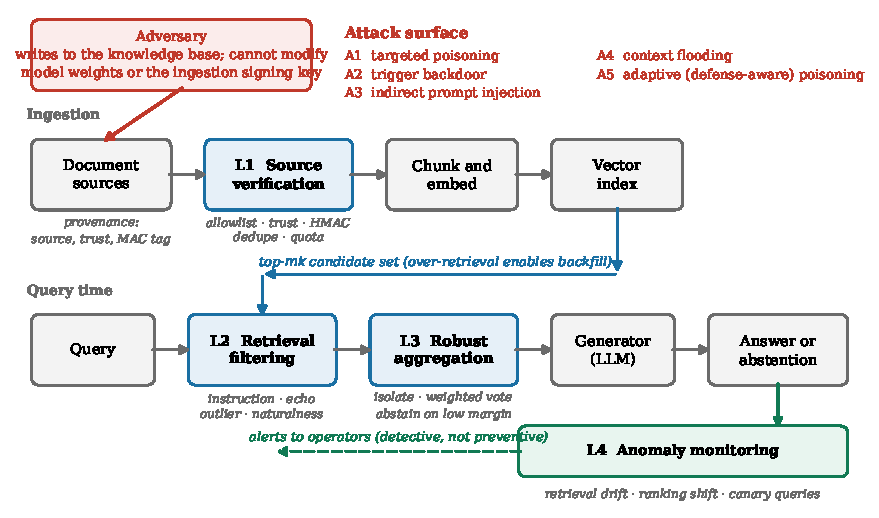
\includegraphics[width=0.78\textwidth]{figures/fig1_architecture.pdf}
\caption{Pipeline, attack entry point, and the four switchable controls. The figure shows
adversary $\AdvU$, which holds no signing key; adversary $\AdvC$ additionally holds the key of
one authorized publisher, so its documents pass Layer~1 by construction.}
\label{fig:architecture}
\end{figure*}

\subsection{Adversaries}

We distinguish two adversaries that differ in exactly one capability.

\emph{Adversary $\AdvU$, the unauthorized writer}, can write to the knowledge base through an
untrusted connector or a compromised upload account with no signing authority. It cannot read
or forge any publisher's key. This is the adversary that provenance-based defenses assume.

\emph{Adversary $\AdvC$, the compromised authorized publisher}, holds the signing key of one
publisher among the $P$ that the deployment authorizes. Its documents carry tags that verify,
so no allowlist, trust score, or tag check can exclude them. $\AdvC$ models key theft, a
malicious insider at a contributing publisher, and a publisher whose own upstream has been
subverted. It holds no other publisher's key, and because the tag covers identity, source, and
content jointly, it cannot alter documents published by others.

Both adversaries know the defense, including its architecture, filters, and thresholds, and
both know the target questions. Neither can modify the generator, the retriever, or the
ingestion service, or observe other users' queries. The budget is the number of documents $b$
inserted per target question. Results for authenticated configurations are under $\AdvU$
unless stated; Section~\ref{sec:compromise} reports them under $\AdvC$. Replay, freshness, and
revocation are out of scope.

We operationalize target knowledge by giving the adversary the full benchmark question list
and attacking every question. This is batch poisoning with complete benchmark access, not a
model of discovering unknown production queries. Two goals are distinguished. Under
\emph{substitution} the adversary chooses a target answer $a^{*}$ and succeeds when $a^{*}$
appears in the response; each target is assigned the answer of a different benchmark question,
excluding assignments that overlap the gold answer. Under \emph{suppression} the adversary
succeeds when the correct answer does not appear.

\subsection{Attack Instantiations}
\label{sec:adaptive}

Table~\ref{tab:attacks} lists the five attack families. A1--A4 reproduce published static
constructions and make no attempt to evade detection. Each has a syntactic tell: A1 and A4
open with the target question, A3 contains an imperative override, and A2 a low-entropy
trigger.

\begin{table}[t]
\centering
\footnotesize
\caption{Attack families evaluated.}
\label{tab:attacks}
\begin{tabularx}{\columnwidth}{@{}l>{\raggedright\arraybackslash}X@{}}
\toprule
\textbf{ID} & \textbf{Mechanism and goal}\\
\midrule
A1 & Targeted poisoning: target query concatenated with an adversarial
     statement~\cite{zou2024}. Substitution.\\
A2 & Trigger backdoor: passage dormant until a rare trigger is appended to the
     query~\cite{xue2024badrag,chaudhari2024phantom}. Substitution.\\
A3 & Indirect prompt injection: retrievable passage carrying an instruction override,
     optionally obfuscated~\cite{greshake2023}. Substitution.\\
A4 & Context flooding: query-matching passages with no answer crowd evidence out of the
     top-$k$~\cite{shafran2024jamming}. Suppression.\\
A5 & Rewriting adversary: declarative, instruction-free, naturally padded passages under a
     claimed trusted source (this section). Substitution.\\
\bottomrule
\end{tabularx}
\end{table}

A5 pursues the same goal as A1 but is written against the deployed stack. It combines six
independently switchable techniques so that its success can be attributed: (E1) the claim is
a declarative sentence built from the query's content words and never reproduces the
question; (E2) the payload asserts the answer instead of instructing the generator; (E3) the
claim is embedded in fluent, topically neutral prose; (E4) the padding keeps similarity to the
query below the near-duplicate threshold and the passage near the corpus centroid; (E5) the
document claims a source identifier that the deployment trusts; and (E6) the $b$ documents use
distinct text and identifiers, so deduplication retains them and an identifier-counting
aggregator treats them as separate support. A5 uses no gradient information and no queries to
the deployed system. It is a manually specified rewriting adversary, cheap to implement, and
is not claimed to be the strongest adaptive attack. Under $\AdvC$ the same documents are
signed with the compromised publisher's key.

\section{Pipeline Controls}
\label{sec:architecture}

Each control implements a common interface with optional hooks for ingestion, retrieval,
generation, and response, so any subset can be enabled without altering the retriever, the
generator, or the evaluation protocol.

\subsection{Layer 1: Source Verification}
\label{sec:layer1}

Layer~1 decides what may enter the index. It applies, in order: a source allowlist; a minimum
trust threshold $\theta_{\mathrm{trust}}$ on the server-assigned score; verification of an
HMAC-SHA256 tag~\cite{krawczyk1997hmac} recomputed over the envelope of Eq.~(\ref{eq:env});
content-hash deduplication; and a per-source document quota. The source identifier is a
caller-supplied claim. Allowlists and trust policy constrain how a claimed identifier is
treated but do not authenticate the publisher; only a valid tag does. Requiring tags without a
runtime verification key is rejected at construction rather than degrading to a no-op.

HMAC is a symmetric primitive, so the experiments model a registry in which the ingestion
service holds one key per authorized publisher. On a successful check Layer~1 records which
key verified the document as $\mathrm{signer}(d)$. That field is written by the service and is
never read from caller-supplied metadata. Keys are generated per run, held in memory, and
absent from source, configuration, and result files. The registry assumes that the verifying
service is itself trusted, since it could forge any publisher's tag. A deployment that cannot
make that assumption needs public-key signatures, with the signer identity a certified public
key. Nothing below depends on the primitive; it depends on an authenticated publisher identity.

\subsection{Layer 2: Retrieval Filtering}

Layer~2 scores every candidate in $R(q)$ with four detectors that target different mechanisms:
an instruction-pattern filter applied after Unicode normalization and removal of invisible
characters; a query-echo filter on bigram overlap and interrogative openings; a
similarity-outlier filter for near-duplicates of the query and for centroid outliers; and a
naturalness filter on gibberish ratio, repetition, and character entropy. Each statistic is
divided by its own hand-set decision threshold $\theta_i$,
\begin{equation}
\mathrm{susp}(c, q) = \max_i\ \mathrm{clip}\!\left(\frac{\mathrm{stat}_i(c, q)}{\theta_i},\, 0,\, 1.5\right),
\label{eq:suspicion}
\end{equation}
and a candidate is dropped when $\mathrm{susp}(c,q) \ge \tau$, with $\tau = 1$ by default. The
score is threshold-normalized, not calibrated, and is not a probability.

\subsection{Layer 3: Provenance-Weighted Aggregation}

Layer~3 replaces the single stuffed-context generation with isolate-then-aggregate in the
manner of RobustRAG~\cite{xiang2024robustrag}. Each surviving passage $j$ is used alone to
produce a candidate answer; abstentions are discarded. Each answer receives the weight
\begin{equation}
w_j = \omega_j \cdot \max(\rho_j, \rho_{\min})^{\gamma} \cdot \phi_j ,
\label{eq:wj}
\end{equation}
where $\omega_j$ is the source trust of the supporting passage, $\rho_j \in [0,1]$ the fraction
of addressable query terms it contains, $\gamma = 2$, and $\phi_j \in \{0.2, 1\}$ a penalty
applied when Layer~2 flagged the passage. Answers are grouped by Jaccard overlap of their
content tokens, and a group $g$ is scored by
\begin{equation}
W_{\mathrm{id}}(g) = \Big(\sum_{j \in g} w_j\Big)\cdot
\big(1 + \beta\,(|\mathrm{docs}(g)| - 1)\big),
\label{eq:weight}
\end{equation}
where $\mathrm{docs}(g)$ is the set of distinct document identifiers in $g$ and $\beta = 0.25$
is a redundancy bonus. The layer returns the top group's answer only if that group clears a
minimum weight $w_{\min} = 0.1$ and exceeds the runner-up by a margin $\mu = 1.25$; otherwise
it abstains. We refer to Eq.~(\ref{eq:weight}) as \emph{identifier counting}. It treats
agreement across distinct identifiers as support without verifying that the identifiers
correspond to distinct parties.

\subsection{Layer 4: Monitoring}
\label{sec:l4}

Layer~4 is detective. It reports when the Jensen--Shannon divergence~\cite{lin1991divergence}
between consecutive windows of retrieved chunk identifiers exceeds a threshold, re-runs
registered benchmark queries, and executes canary queries. It never rewrites an answer or
removes a document, and is included so that the ablation states what detection does and does
not contribute.

\section{A Per-Principal Contribution Cap}
\label{sec:cap}

Equation~(\ref{eq:weight}) rewards the one quantity an adversary controls for free. Writing
the same claim into $b$ documents adds up to $b$ weighted terms to the sum and multiplies the
redundancy factor by up to $1 + \beta(b-1)$, at the cost of $b$ uploads. We replace the unit
over which agreement is counted and cap what any one party can contribute.

\subsection{The Principal and Its Binding}

A principal is useful only if the adversary cannot mint new ones, which rules out every
attribute the uploader chooses. For a passage $j$ we define
\begin{equation}
\prin(j) = \mathrm{signer}(\mathrm{doc}(j)),
\label{eq:indkey}
\end{equation}
the identity of the key whose tag Layer~1 verified. Three properties matter. First,
$\mathrm{signer}$ is written by Layer~1 after a successful check, so a submitter cannot assert
that its document was verified. Second, a document with a tag that no configured key validates
takes the single value $\bot_{\mathrm{unver}}$ and a document with no tag takes the single
value $\bot_{\mathrm{uns}}$, so all unsigned documents form one principal and an
unauthenticated adversary gains nothing from volume. Third, the registry maps each key to one
publisher identity, so a key holder is confined to its own principal whatever else it writes.

The attributes excluded matter as much as the one kept. The envelope of Eq.~(\ref{eq:env})
does not cover an author field, so a key holder may vary the author and still verify. The
source is covered by the tag, so no third party can rewrite it, but the holder of a valid key
chooses it before signing. Coverage by a signature protects an attribute against third
parties, not against the signer. An earlier form of our own rule grouped on signer, source,
and author; Section~\ref{sec:res:binding} measures why that is wrong.

\subsection{Capped Aggregation}

Let $K(g) = \{\prin(j) : j \in g\}$ be the principals present in group $g$. The group score
becomes
\begin{equation}
\begin{split}
W_{\mathrm{cap}}(g) ={}& \Big(\sum_{p \in K(g)} \Big[\max_{j:\,\prin(j) = p} w_j
 + \delta \!\!\sum_{\substack{j:\,\prin(j) = p\\ j \neq j_p^{\star}}}\!\! w_j \Big]\Big)\\
 &\cdot \big(1 + \beta\,(|K(g)| - 1)\big),
\end{split}
\label{eq:indweight}
\end{equation}
where $j_p^{\star}$ is the strongest passage of principal $p$ in $g$ and $\delta \in [0,1]$
controls how much further evidence from an already-counted principal contributes. We use
$\delta = 0$ throughout. Setting $\delta = 1$ and $\prin(j) = \mathrm{doc}(j)$ recovers
Eq.~(\ref{eq:weight}) exactly, so identifier counting is the special case in which every
document is assumed to be its own party; it is the control arm in every experiment.
Algorithm~\ref{alg:cap} gives the procedure.

\begin{algorithm}[t]
\caption{Isolate-then-aggregate with a per-principal cap}
\label{alg:cap}
\begin{algorithmic}[1]
\Require query $q$; passages $C$; generator $G$; margin $\mu$; minimum weight $w_{\min}$;
bonus $\beta$; discount $\delta$
\Ensure answer or abstention
\State $I \gets \emptyset$
\ForAll{$c \in C$}
  \State $a_c \gets G(q, \{c\})$ \Comment{one passage at a time}
  \If{$a_c$ is an abstention} \State \textbf{continue} \EndIf
  \State $w_c \gets$ weight from Eq.~(\ref{eq:wj})
  \State $p_c \gets \mathrm{signer}(\mathrm{doc}(c))$ \Comment{set by Layer~1, never by the caller}
  \State $I \gets I \cup \{(a_c, w_c, p_c)\}$
\EndFor
\State $\mathcal{G} \gets$ group $I$ by Jaccard overlap of answer tokens
\ForAll{$g \in \mathcal{G}$}
  \State $S \gets 0$
  \ForAll{principals $p$ present in $g$}
     \State $w^{\star} \gets \max\{w_c : p_c = p\}$
     \State $r \gets \sum\{w_c : p_c = p\} - w^{\star}$
     \State $S \gets S + w^{\star} + \delta\, r$
  \EndFor
  \State $W(g) \gets S \cdot (1 + \beta(|K(g)| - 1))$
\EndFor
\State rank $\mathcal{G}$ by $W$ as $g_1, g_2, \dots$
\If{$\mathcal{G} = \emptyset$ \textbf{or} $W(g_1) < w_{\min}$ \textbf{or} $W(g_1) < \mu\, W(g_2)$}
  \State \Return \textsc{abstain}
\EndIf
\State \Return representative answer of $g_1$
\end{algorithmic}
\end{algorithm}

\subsection{What the Cap Guarantees}

The following bound is immediate from Eq.~(\ref{eq:indweight}) and states exactly what the
mechanism provides.

\emph{Property 1 (bounded contribution).} Let $\delta = 0$ and let an adversary control a set
$A$ of principals. For any answer group $g$ and any number of adversarial passages in $g$, the
adversary's contribution to the sum in Eq.~(\ref{eq:indweight}) is at most
$\sum_{p \in A} \max_{j:\,\prin(j)=p} w_j \le \sum_{p \in A} \omega_p$, and its contribution to
$|K(g)|$ is at most $|A|$. In particular, for $\AdvC$ with $|A| = 1$, the score of a group
supported only by the adversary is at most $\omega_p$ for every budget $b$, whereas under
Eq.~(\ref{eq:weight}) it can reach $k' \omega_p (1 + \beta(k'-1))$ when $k' \le \min(b, k)$ of
its passages are retrieved.

The bound follows because $\rho_j \le 1$ and $\phi_j \le 1$ give $w_j \le \omega_j$, and each
principal contributes one term. It holds whether the party is unsigned, carries an
unverifiable tag, or holds a valid key, so it applies to $\AdvC$ as well as $\AdvU$.

The property is a statement about weight and nothing more. It does not say that two principals
reasoned independently, consulted different evidence, or told the truth, which is why we name
the rule a cap and not an independence test. Two limits follow from its form. With $b = 1$
the adversary has one passage under either rule, so Eqs.~(\ref{eq:weight})
and~(\ref{eq:indweight}) coincide and the cap cannot help. And the cap acts on the passages
that reach aggregation: if the adversary's passages occupy the candidate set, the honest
principal is absent and cannot outweigh anything. Section~\ref{sec:compromise} measures both.
The rule adds no model call and no retrieval cost.

\section{Experimental Design}
\label{sec:experiments}

\subsection{Corpora and Models}

We evaluate on SQuAD~\cite{rajpurkar2016squad} (300 documents, 300 questions),
HotpotQA~\cite{yang2018hotpotqa} in its distractor configuration (1,999 documents, 200
questions), and a bundled 30-document toy corpus that allows the study to be reproduced
offline. HotpotQA's distractor paragraphs give the retrieval filter a supply of topically
adjacent non-answers, so a low false-positive rate is not obtained for the wrong reason. Both
public datasets are pinned to immutable repository revisions recorded in the artifact
manifest, and all runs use the validation split.

Passages and queries are embedded with
\texttt{all-MiniLM-L6-v2}~\cite{reimers2019sbert,wang2020minilm} and indexed with exact
inner-product search~\cite{johnson2021faiss}. The main factorial uses a deterministic
generator that answers extractively from the passage most lexically aligned with the question
and, unless hardened, follows instructions in retrieved text. This makes outcomes repeatable
and isolates the pipeline from model variance, but the generator is credulous by
construction, so absolute attack rates are an upper bound and are not evidence of
model-independent behavior.

A confirmation on SQuAD uses \texttt{qwen2.5:7b}~\cite{qwen257bmodelcard} and
\texttt{llama3.1:8b}~\cite{llama318bmodelcard} served locally through an OpenAI-compatible
endpoint, with 100 validation questions, one seed, temperature 0, and a 128-token limit. No
hosted commercial model was evaluated.

\subsection{Metrics}
\label{sec:metrics}

Attack success rate (ASR) is the fraction of attacked queries that meet the adversary's goal.
For suppression, unconditional ASR is inflated by the pipeline's own errors, because a query
the system would have answered wrongly is counted as suppressed. We therefore also report
\emph{attributable ASR}, restricted to queries that the same configuration answered correctly
in a clean run, and we run every configuration once without an attack to establish that
baseline. We further report clean accuracy and abstention rate, poison retrieval and use
rates, and the retrieval filter's true- and false-positive rates with threshold-free area
under the ROC curve~\cite{davis2006prc,saito2015prc}. Ground-truth poison labels are used only
for scoring.

Correctness and target satisfaction use normalized substring matching, which is lenient. As a
graded check we also compute token F1 between the generated answer and the assigned target
with SQuAD normalization.

Point estimates pool query--seed trials over \nSeeds{} seeds. For the main and
compromised-publisher studies we report 95\% percentile-bootstrap intervals from 2,000
resamples of distinct questions, each retaining its outcomes across seeds; the intervals
quantify question-sampling uncertainty conditional on those seeds. Served-model results use
Wilson intervals~\cite{wilson1927,brown2001interval} for marginal rates and paired statistics
for the comparison of aggregation rules.

\subsection{Configurations}

We compare the undefended pipeline, each layer alone (L1--L4), the full stack, and the full
stack with authenticated ingestion, in which a publisher registry tags the legitimate corpus
and Layer~1 requires a valid tag. Unless stated, $k = 3$, $m = 10$, and
$\theta_{\mathrm{trust}} = 0.6$; the server assigns trust 0.8 to the legitimate source and 0.5
to unmapped identifiers. The adversary uses one document per target for A1--A3, five for A4,
and three for A5. In the compromised-publisher study the legitimate corpus is dealt round
robin across $P = 8$ publisher keys, $\AdvC$ holds one of them, and $b \in \{1,2,3,5,8\}$.
The diversity control varies $P$ from 1 to 16 at $b = 5$, and the binding study compares three
grouping attributes at $b = 5$. Supporting studies cover the evasion ablation, budget and
threshold sweeps, over-retrieval, the ingestion-control ladder, and generator hardening.

The code, configurations, seeds, model and dataset revisions, and the aggregate and hashed
per-query outcomes are released; tables, figures, and the numeric macros in this text are
regenerated from that bundle. The supplemental material gives the corpus statistics, the
supporting ablations, and the full served-model results as Tables~V--X and Figs.~4 and~5.

\section{Results}
\label{sec:results}

\subsection{Unauthorized Writer: Content Controls and Authentication}
\label{sec:res:adaptive}

Table~\ref{tab:main} gives the full grid under adversary $\AdvU$. Undefended, every attack
succeeds: pooled over the four static attacks, ASR is \asrStaticSquadnone{} on SQuAD and
\asrStaticHotpotqanone{} on HotpotQA, and the rewriting adversary reaches
\asrAdaptiveSquadnone{} and \asrAdaptiveHotpotqanone{}. Clean accuracy is
\cleanAccSquadnone{} on SQuAD but \cleanAccHotpotqanone{} on HotpotQA, because the
deterministic generator answers from a single passage and HotpotQA questions require two. That
low ceiling is why the attributable rate is needed. Under the full defense, context flooding
has a raw ASR of \asrFloodingSquadfull{} on SQuAD and an attributable ASR of
\casrFloodingSquadfull{}: the raw figure measures the pipeline's own error rate.

\begin{table*}[t]
\begin{adjustwidth}{-\extralength}{0cm}
\centering
\footnotesize
\setlength{\tabcolsep}{3pt}
\caption{Attack success by defense configuration.\label{tab:main}}
\begin{tabularx}{\textwidth}{>{\raggedright\arraybackslash}p{1.5in}>{\centering\arraybackslash}X>{\centering\arraybackslash}X>{\centering\arraybackslash}X>{\centering\arraybackslash}X>{\centering\arraybackslash}X>{\centering\arraybackslash}X}
\toprule
\textbf{Configuration} & \textbf{\shortstack{Poisoned\\RAG}} & \textbf{\shortstack{Trigger\\backdoor}} & \textbf{\shortstack{Prompt\\injection}} & \textbf{\shortstack{Context\\flooding}} & \textbf{\shortstack{Adaptive\\poisoning}} & \textbf{\shortstack{Clean\\accuracy}}\\
\midrule
\multicolumn{7}{l}{\textit{SQuAD}}\\
No defense & 0.99 \tiny(0.99) & 0.85 \tiny(0.89) & 0.96 \tiny(0.97) & 1.00 \tiny(1.00) & 0.81 \tiny(0.83) & 0.62\\
L1 source verification & 0.01 \tiny(0.01) & 0.01 \tiny(0.01) & 0.01 \tiny(0.01) & 0.38 \tiny(0.00) & 0.81 \tiny(0.83) & 0.62\\
L2 retrieval filtering & 0.01 \tiny(0.01) & 0.01 \tiny(0.01) & 0.01 \tiny(0.01) & 0.42 \tiny(0.04) & 0.81 \tiny(0.83) & 0.61\\
L3 robust aggregation & 0.91 \tiny(0.85) & 0.84 \tiny(0.86) & 0.00 \tiny(0.00) & 1.00 \tiny(0.99) & 0.84 \tiny(0.86) & 0.52\\
L4 monitoring & 0.99 \tiny(0.99) & 0.85 \tiny(0.89) & 0.96 \tiny(0.97) & 1.00 \tiny(1.00) & 0.81 \tiny(0.83) & 0.62\\
Full defense & 0.00 \tiny(0.00) & 0.00 \tiny(0.00) & 0.00 \tiny(0.00) & 0.49 \tiny(0.00) & 0.82 \tiny(0.83) & 0.51\\
Full + HMAC auth. & 0.00 \tiny(0.00) & 0.00 \tiny(0.00) & 0.00 \tiny(0.00) & 0.49 \tiny(0.00) & 0.00 \tiny(0.00) & 0.51\\
\multicolumn{7}{l}{\textit{HotpotQA}}\\
No defense & 0.96 \tiny(0.95) & 0.93 \tiny(0.95) & 0.95 \tiny(0.96) & 1.00 \tiny(1.00) & 0.95 \tiny(0.97) & 0.25\\
L1 source verification & 0.00 \tiny(0.01) & 0.00 \tiny(0.01) & 0.00 \tiny(0.01) & 0.75 \tiny(0.00) & 0.95 \tiny(0.97) & 0.25\\
L2 retrieval filtering & 0.00 \tiny(0.01) & 0.01 \tiny(0.01) & 0.00 \tiny(0.01) & 0.74 \tiny(0.00) & 0.96 \tiny(0.97) & 0.26\\
L3 robust aggregation & 0.94 \tiny(0.89) & 0.92 \tiny(0.95) & 0.01 \tiny(0.01) & 0.99 \tiny(1.00) & 0.96 \tiny(0.98) & 0.19\\
L4 monitoring & 0.96 \tiny(0.95) & 0.93 \tiny(0.95) & 0.95 \tiny(0.96) & 1.00 \tiny(1.00) & 0.95 \tiny(0.97) & 0.25\\
Full defense & 0.01 \tiny(0.01) & 0.00 \tiny(0.01) & 0.01 \tiny(0.01) & 0.81 \tiny(0.00) & 0.90 \tiny(0.95) & 0.19\\
Full + HMAC auth. & 0.01 \tiny(0.01) & 0.00 \tiny(0.01) & 0.01 \tiny(0.01) & 0.81 \tiny(0.00) & 0.01 \tiny(0.01) & 0.19\\
\multicolumn{7}{l}{\textit{Toy corpus}}\\
No defense & 0.60 \tiny(0.60) & 1.00 \tiny(1.00) & 1.00 \tiny(1.00) & 0.87 \tiny(0.87) & 0.46 \tiny(0.46) & 1.00\\
L1 source verification & 0.00 \tiny(0.00) & 0.00 \tiny(0.00) & 0.00 \tiny(0.00) & 0.00 \tiny(0.00) & 0.46 \tiny(0.46) & 1.00\\
L2 retrieval filtering & 0.00 \tiny(0.00) & 0.00 \tiny(0.00) & 0.00 \tiny(0.00) & 0.10 \tiny(0.00) & 0.52 \tiny(0.47) & 0.90\\
L3 robust aggregation & 0.46 \tiny(0.46) & 1.00 \tiny(1.00) & 0.00 \tiny(0.00) & 0.87 \tiny(0.87) & 1.00 \tiny(1.00) & 1.00\\
L4 monitoring & 0.60 \tiny(0.60) & 1.00 \tiny(1.00) & 1.00 \tiny(1.00) & 0.87 \tiny(0.87) & 0.46 \tiny(0.46) & 1.00\\
Full defense & 0.00 \tiny(0.00) & 0.00 \tiny(0.00) & 0.00 \tiny(0.00) & 0.10 \tiny(0.00) & 0.94 \tiny(0.94) & 0.90\\
Full + HMAC auth. & 0.00 \tiny(0.00) & 0.00 \tiny(0.00) & 0.00 \tiny(0.00) & 0.10 \tiny(0.00) & 0.00 \tiny(0.00) & 0.90\\
\bottomrule
\end{tabularx}
\par\vspace{3pt}
\noindent\parbox{\linewidth}{\footnotesize Pooled over query-seed trials. Each cell reads \emph{raw} (\emph{attack-attributable}), the latter restricted to queries the same configuration answered correctly with no adversary present. The two diverge only for the suppression attack, whose raw rate absorbs the pipeline's own error rate; this is most visible on HotpotQA, where multi-hop questions depress clean accuracy. Figure~\ref{fig:bars} shows the observed minimum-to-maximum range across seeds. The last column is clean accuracy on the unattacked corpus, i.e.\ the utility cost of the configuration.}
\end{adjustwidth}
\end{table*}


\emph{Static attacks.} Ingestion verification and retrieval filtering each reduce pooled
static attributable success on SQuAD to \casrStaticSquadLOne{} and \casrStaticSquadLTwo{}, and
the full stack to \casrStaticSquadfull{}. Aggregation alone leaves
\casrStaticSquadLThree{} and carries the largest clean-accuracy cost of any single layer
(\cleanAccSquadnone{} to \cleanAccSquadLThree{}), since its margin rule abstains when
competing groups have similar weight. Monitoring alone changes nothing
(\casrStaticSquadLFour{}), as a detective control should.

\emph{Rewriting adversary.} Against A5 the picture reverses. Attributable success on SQuAD is
\casrAdaptiveSquadnone{} undefended and \casrAdaptiveSquadfull{} under the full stack. The
retrieval filter separates static payloads almost perfectly (area under the ROC curve
\detectionAurocPoisonedragSquad{} for A1 on SQuAD) and fails on A5
(\detectionAurocAdaptiveSquad{}), with a false-positive rate of \detectionFprSquad{} on clean
traffic. Removing one technique at a time (Table~VI of the supplement) shows that three are
necessary: the rewriting (E1, E2) defeats the filter and the claimed source (E5) passes the
trust threshold. Padding, dilution, and identifier diversification (E3, E4, E6) are not
needed against this stack. Aggregation alone does not lower attributable A5 success on any corpus
(\casrAdaptiveSquadLThree{} on SQuAD, \casrAdaptiveHotpotqaLThree{} on HotpotQA) and raises it
from \casrAdaptiveToynone{} to \casrAdaptiveToyLThree{} on the toy corpus, because identifier
counting credits the adversary's $b$ distinct identifiers as support. Mean target token F1 on SQuAD is \targetTokenFAdaptiveSquadNone{} undefended and
\targetTokenFAdaptiveSquadFull{} under the full stack, so the graded measure agrees with the
binary one. These outcomes describe the tested detectors and payloads; they do not show that
every content filter fails.

\emph{Ingestion controls.} Against a static adversary, a trust threshold takes success from
\provOpenStatic{} to \provTrustonlyStatic{}. Against A5 the trust threshold and the allowlist
do nothing (\provOpenAdaptive{}, \provTrustonlyAdaptive{}, \provAllowlistAdaptive{}), because
the adversary claims an accepted source identifier. A per-source quota of 1.5 times the
legitimate corpus reduces A5 success to \provQuotaAdaptive{} on SQuAD and leaves
\provQuotaAdaptiveHotpot{} on HotpotQA, where the campaign fits inside the allowance: a quota
prices a mass campaign and is blind to a targeted one. Requiring a valid tag reduces A5
success to \provSignedAdaptive{}, and in the main grid to \casrAdaptiveSquadfullsigned{} on
SQuAD and \casrAdaptiveHotpotqafullsigned{} on HotpotQA with clean accuracy unchanged; target
F1 falls to \targetTokenFAdaptiveSquadFullsigned{}. Under $\AdvU$, then, authenticated
ingestion is the only evaluated control that stops the rewriting adversary.

\subsection{Compromised Authorized Publisher}
\label{sec:compromise}

We now grant the adversary the key of one authorized publisher among eight and change nothing
else. Its documents pass the allowlist, the trust threshold, and the tag check.
Table~\ref{tab:compromise} and Fig.~\ref{fig:compromise} report the results. The magnitudes
are for the deterministic generator and should be read as the amount of corroboration the
adversary can manufacture. What does not depend on the generator is the admission result: a
correctly tagged document from an authorized source passes ingestion whatever the generator
later does with it.

\begin{table*}[t]
\begin{adjustwidth}{-\extralength}{0cm}
\centering
\footnotesize
\setlength{\tabcolsep}{4pt}
\caption{Attack success under a compromised publisher.\label{tab:compromise}}
\begin{tabular}{llrrr}
\toprule
Corpus & Budget & Document identifier & Verified signer & $n_0$ \\
\midrule
SQuAD & $b=1$ & 0.65 [0.58, 0.72] & 0.65 [0.58, 0.72] & 462 \\
 & $b=2$ & 0.82 [0.76, 0.87] & 0.70 [0.63, 0.77] & 462 \\
 & $b=3$ & 0.82 [0.76, 0.87] & 0.63 [0.56, 0.69] & 462 \\
 & $b=5$ & 0.83 [0.78, 0.88] & 0.59 [0.53, 0.65] & 462 \\
 & $b=8$ & 0.85 [0.80, 0.90] & 0.77 [0.72, 0.83] & 462 \\
\addlinespace
HotpotQA & $b=1$ & 0.64 [0.52, 0.77] & 0.64 [0.51, 0.78] & 123 \\
 & $b=2$ & 0.84 [0.72, 0.93] & 0.84 [0.73, 0.93] & 123 \\
 & $b=3$ & 0.83 [0.71, 0.93] & 0.71 [0.60, 0.81] & 123 \\
 & $b=5$ & 0.85 [0.75, 0.95] & 0.70 [0.59, 0.81] & 123 \\
 & $b=8$ & 0.92 [0.84, 0.98] & 0.86 [0.76, 0.95] & 123 \\
\addlinespace
\bottomrule
\end{tabular}
\par\vspace{3pt}
\noindent\parbox{\linewidth}{\footnotesize Attack-attributable success with 95\% question-cluster bootstrap intervals, under adversary $\mathcal{C}$, which holds one authorized publisher's signing key. Signed ingestion admits its documents by construction, so the columns differ only in the unit agreement is counted over. $n_0$ is the pooled clean-correct denominator across three seeds. Abstention on attacked queries rises with the cap; it is reported in the text.}
\end{adjustwidth}
\end{table*}

\begin{figure*}[t]
\centering
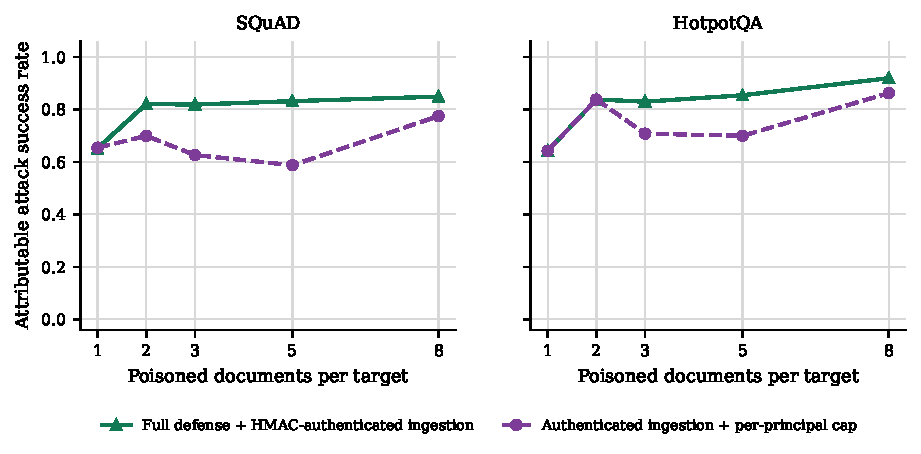
\includegraphics[width=0.8\textwidth]{figures/fig4_compromise.pdf}
\caption{Attributable attack success against the upload budget under adversary $\AdvC$, for
identifier counting (solid) and the per-principal cap (dashed), both with authenticated
ingestion.}
\label{fig:compromise}
\end{figure*}

\emph{Authentication contributes nothing once a key is held.} At $b = 3$, attributable success
under the authenticated configuration rises from \casrAdaptiveSquadfullsigned{} to
\compromiseSignedSquadBThree{}
(\compromiseCIFullsignedSquadBThreeLow{}--\compromiseCIFullsignedSquadBThreeHigh{}) on SQuAD
and from \casrAdaptiveHotpotqafullsigned{} to \compromiseSignedHotpotqaBThree{}
(\compromiseCIFullsignedHotpotqaBThreeLow{}--\compromiseCIFullsignedHotpotqaBThreeHigh{}) on
HotpotQA; on SQuAD that is the level of the undefended pipeline (\casrAdaptiveSquadnone{}). The protection measured in
Section~\ref{sec:res:adaptive} is therefore a property of the assumption that no authorized
publisher is adversarial. This negative result applies to our own best-performing
configuration.

\emph{Identifier counting sells the adversary an escalation.} Under $\AdvC$ attributable
success grows with the number of documents written: on SQuAD from \compromiseSignedSquadBOne{}
at $b = 1$ to \compromiseSignedSquadBEight{} at $b = 8$, and on HotpotQA from
\compromiseSignedHotpotqaBOne{} to \compromiseSignedHotpotqaBEight{}. The growth is bought with
uploads, not with any further compromise.

\emph{The cap removes part of that escalation.} With Eq.~(\ref{eq:indweight}), attributable
success at $b = 5$ on SQuAD is \compromiseSignedIndependentSquadBFive{}
(\compromiseCIFullsignedindependentSquadBFiveLow{}--\compromiseCIFullsignedindependentSquadBFiveHigh{})
against \compromiseSignedSquadBFive{}
(\compromiseCIFullsignedSquadBFiveLow{}--\compromiseCIFullsignedSquadBFiveHigh{}) under
identifier counting. The intervals are disjoint. On HotpotQA the corresponding values are
\compromiseSignedIndependentHotpotqaBFive{}
(\compromiseCIFullsignedindependentHotpotqaBFiveLow{}--\compromiseCIFullsignedindependentHotpotqaBFiveHigh{})
against \compromiseSignedHotpotqaBFive{}
(\compromiseCIFullsignedHotpotqaBFiveLow{}--\compromiseCIFullsignedHotpotqaBFiveHigh{}); the
intervals overlap because the attributable rate there is conditioned on the roughly one fifth
of questions the generator answers correctly, so the HotpotQA reduction is directional and the
SQuAD result carries the claim. Clean accuracy is unaffected
(\compromiseCleanAccSignedIndependentSquadBFive{} against
\compromiseCleanAccSignedSquadBFive{}). The reduction is paid for in abstention on attacked
queries, which rises from \compromiseAbstainSignedSquadBFive{} to
\compromiseAbstainSignedIndependentSquadBFive{} on SQuAD: denied a fabricated majority, the
layer declines to answer more often. That is the intended failure direction, and it is a cost.
The cap does not restore the protection that authentication provides against $\AdvU$; more
than half of the attacks still succeed.

\emph{The benefit is bounded at both ends.} At $b = 1$ the two rules coincide
(\compromiseSignedSquadBOne{} and \compromiseSignedIndependentSquadBOne{} on SQuAD), as
Section~\ref{sec:cap} predicts. At $b = 8$ the advantage narrows to
\compromiseSignedIndependentSquadBEight{} against \compromiseSignedSquadBEight{}: at high
budgets the adversary's passages displace genuine evidence during retrieval, so the honest
principal is often absent before aggregation is reached. The cap complements retrieval-stage
controls and does not replace them.

\subsection{The Gain Comes From Denying Volume}

The cap is motivated by the intuition that honest evidence is attested by several publishers
while the adversary is one. Fig.~\ref{fig:diversity} tests that explanation by holding $b = 5$
and varying the number of publishers contributing the corpus from one to sixteen. On SQuAD the
capped rate is \diversitySignedIndependentSquadPOne{} with one publisher and
\diversitySignedIndependentSquadPOneSix{} with sixteen, against
\diversitySignedSquadPOneSix{} under identifier counting; on HotpotQA the capped rates are
\diversitySignedIndependentHotpotqaPOne{} and \diversitySignedIndependentHotpotqaPOneSix{}.
The effect does not depend on publisher diversity. The operative mechanism is the bound of
Property~1 on one party's weight, not a corroboration bonus accruing to honest evidence. This
narrows the claim: a deployment should not expect the benefit to grow with the number of
publishers it authorizes.

\begin{figure*}[t]
\centering
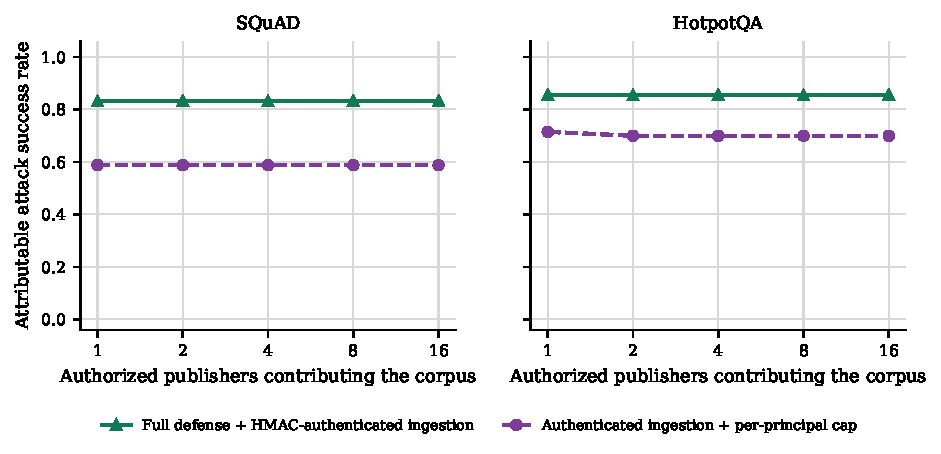
\includegraphics[width=0.8\textwidth]{figures/fig5_diversity.pdf}
\caption{Attributable attack success against the number of authorized publishers contributing
the corpus, at five poisoned documents per target under adversary $\AdvC$.}
\label{fig:diversity}
\end{figure*}

\subsection{Attacking the Binding of the Principal}
\label{sec:res:binding}

A rule that groups evidence by provenance is only as strong as the binding of the attribute it
groups on, so we attack the binding directly. $\AdvC$ varies the author label on every
document it writes. The envelope does not cover the author, so the documents still verify.
Varying the source instead is self-defeating for the adversary, because the allowlist rejects
an unfamiliar label before aggregation sees the document.

Table~\ref{tab:binding} compares identifier counting, a principal of (signer, source, author),
and the signer-only principal of Eq.~(\ref{eq:indkey}). Against a fixed-metadata adversary the
two principals behave identically, so an evaluation that omits this attack cannot tell them
apart. Against the varying adversary, the principal that includes the author collapses to
identifier counting: one key mints one principal per document and the cap applies to nothing.
The signer-only principal is unchanged, because the service assigns that identity from the key
that verified the document and the adversary holds one key. An aggregation rule of this kind
should be stated together with the binding of every attribute it groups on and tested against
an adversary permitted to vary each of them.

\begin{table}[t]
\centering
\footnotesize
\setlength{\tabcolsep}{4pt}
\caption{Binding of the grouping attribute.\label{tab:binding}}
\begin{tabular}{lrr}
\toprule
Aggregation rule & Fixed metadata & Varies author \\
\midrule
Document identifier & 0.83 (0.08) & 0.83 (0.08) \\
Signer, source, author & 0.59 (0.28) & 0.83 (0.08) \\
Verified signer & 0.59 (0.28) & 0.59 (0.28) \\
\bottomrule
\end{tabular}
\par\vspace{3pt}
\noindent\parbox{\linewidth}{\footnotesize Attributable success with abstention on attacked queries in parentheses, at five poisoned documents per target under adversary $\mathcal{C}$, which holds one authorized publisher's key. The author is not covered by the signing envelope, so varying it costs the adversary nothing. Measured on SQuAD. Pooled over three seeds.}
\end{table}

\subsection{Served-Model Confirmation}
\label{sec:res:local}

On 100 SQuAD questions under $\AdvU$, the full content-based stack lowers raw A5 ASR from 0.38
to 0.29 on Qwen2.5~7B and from 0.33 to 0.21 on Llama~3.1~8B, with attributable ASR changing
from 0.31 to 0.27 and from 0.36 to 0.22. Clean accuracy changes from 0.77 to 0.73 on Qwen and
stays at 0.76 on Llama. The Wilson intervals of the undefended and full configurations overlap
for both models, so this is a directional observation. Layers~1 and~2 reduce the static
attacks to zero in this sample and leave A5 near the undefended rate; aggregation alone
increases prompt-injection ASR on both models (0.30 to 0.36 on Llama, 0.13 to 0.37 on Qwen),
because an instruction in an isolated passage still shapes that passage's answer.
Authenticated ingestion yields zero measured ASR for all three attacks tested on both models,
under $\AdvU$. The served models are far less credulous than the deterministic generator: the
undefended attributable A5 rate is \localCasrQwenNone{} and \localCasrLlamaNone{}, against
\casrAdaptiveSquadnone{} in the main study.

The cap was measured on the same two models in a separate run comparing the undefended
pipeline, the full stack, and the full stack with the cap, on one set of model builds.
Attributable A5 success falls from \localCasrQwenFull{} to \localCasrQwenFullIndependent{} on
Qwen and from \localCasrLlamaFull{} to \localCasrLlamaFullIndependent{} on Llama, with clean
accuracy unchanged (\localCleanAccQwenFullIndependent{} and
\localCleanAccLlamaFullIndependent{}). The two arms retrieve the same passages and issue the
same prompts, so the paired difference is the appropriate statistic: it is
\pairedIndepQwenDelta{} (\pairedIndepQwenLow{}, \pairedIndepQwenHigh{}) on Qwen and
\pairedIndepLlamaDelta{} (\pairedIndepLlamaLow{}, \pairedIndepLlamaHigh{}) on Llama. Across
the \pairedIndepPooledPairs{} model--question pairs the cap prevented
\pairedIndepPooledPrevented{} attacks that succeeded under identifier counting and caused
\pairedIndepPooledCaused{}, an exact McNemar $p$ of \pairedIndepPooledP{}.

The direction is consistent and no regression was observed, which is the behavior the rule is
designed for: it can withdraw weight from a fabricated majority and has no mechanism by which
to manufacture one. Four discordant pairs do not establish the effect, and we do not claim
they do. This run used unsigned ingestion under $\AdvU$, where all unsigned documents form one
principal; the compromised-publisher configuration of Section~\ref{sec:compromise} has not
been run on served models. We therefore report the cap as measured with the deterministic
generator, directionally consistent on served models, and not confirmed by them.

\section{Discussion}
\label{sec:discussion}

\subsection{What Authentication Does and Does Not Buy}

Authentication answers the question of who vouched for a document. Against a writer with no
key, that answer is sufficient, because the honest answer is ``nobody authorized.'' Against an
authorized publisher it is not an obstacle at all. An evaluation of a provenance control that
reports a near-zero poisoning rate has therefore measured its adversary model, and the number
should be reported together with the assumption that produces it. The practical exposure grows
with the number of authorized publishers, since each key is a separate opportunity for
compromise, while the measured protection under $\AdvU$ does not change.

\subsection{Operational Implications}

Bind a versioned document envelope to an authenticated publisher identity and verify it before
indexing; where publishers and the verifier are separately administered, use public-key
signatures. Record at ingestion which key verified each document, and expose only that
service-assigned identity to downstream controls. Where aggregation rewards repeated answers,
count principals whose identity has been proved and not submitter-chosen identifiers, and
accept the additional abstention. Because the cap stops helping once poison displaces genuine
passages at retrieval, pair it with a retrieval-stage limit on the share of a candidate set
that one principal may occupy; we have not evaluated such a limit. Because signing cannot
exclude an authorized adversary, publisher authorization needs per-publisher quotas,
revocation, and monitoring. Content filters remain useful as detection signals for unrewritten
payloads, but their contribution should be measured against rewritten ones and reported with
false-positive and clean-utility costs.

\subsection{Limitations}
\label{sec:limitations}

\emph{Generator.} The main and compromised-publisher studies use a deterministic generator
that is credulous by construction. The served-model confirmation covers two open-weight
models, 100 questions, and one seed, and it does not include adversary $\AdvC$. The cap's
effect on served models is unconfirmed.

\emph{Scale.} The corpora contain 30 to 1,999 documents, with one sentence-transformer
retriever and exact search. We did not evaluate production vector databases, connector
authorization, multi-tenant access control, or large indexes.

\emph{Adversary.} The adversary knows and targets every benchmark question and uses six
manually selected transformations without optimization or feedback. Attacker and defenses
share one codebase. $\AdvC$ holds exactly one key; colluding publishers would raise the bound
of Property~1 in proportion to their number.

\emph{Baselines.} RobustRAG, TrustRAG, RAGShield, and the other systems discussed in
Section~\ref{sec:related} were not reimplemented, so the comparison with them is qualitative.
The identifier-counting control arm is our own aggregation rule, not a reproduction of a
published one.

\emph{Measurement.} Binary success uses substring matching, with token F1 as a graded check
in the main study only. The retrieval score is threshold-normalized and not calibrated.
Intervals condition on three seeds.

\emph{Cryptographic model.} The HMAC registry assumes a trusted verifying service. Replay,
freshness, key rotation, and revocation are not tested, and we do not measure the operational
cost of key management.

\emph{The cap itself.} It bounds weight and does not assess truth, so it cannot distinguish a
well-supported falsehood from a fact. Where every document shares one signer, the partition is
trivial and the rule reduces to taking a single party's strongest passage.

\section{Conclusion}
\label{sec:conclusions}

Authenticated ingestion excluded every poisoned document written by an adversary without a key
and none written by an adversary with one. Granting the adversary a single authorized
publisher's key raised attributable success under the authenticated configuration from
\casrAdaptiveSquadfullsigned{} to \compromiseSignedSquadBThree{} on SQuAD and from
\casrAdaptiveHotpotqafullsigned{} to \compromiseSignedHotpotqaBThree{} on HotpotQA. What
remained exploitable was the unit over which corroboration is counted. Counting agreement over
verified signer identities, with each principal contributing only its strongest passage,
lowered attributable success from \compromiseSignedSquadBFive{} to
\compromiseSignedIndependentSquadBFive{} on SQuAD at five documents per target with clean
accuracy unchanged and more abstention. The benefit vanished at one document, narrowed at
eight, did not depend on publisher diversity, and disappeared when the principal included an
attribute the uploader could choose. On two served models the rule prevented
\pairedIndepPooledPrevented{} attacks and caused \pairedIndepPooledCaused{} in
\pairedIndepPooledPairs{} paired trials, which is consistent in direction and too small to
confirm.

These results do not establish a generally effective defense or behavior at production scale.
They support three narrower statements: a provenance control should be evaluated under an
adversary that holds a valid key; an aggregation rule should count parties whose identity has
been proved; and the attribute that defines a party must be one the adversary cannot choose.

\section*{Acknowledgment}

The authors used Anthropic's Claude, an AI assistant, to support implementation, experiment
orchestration, analysis scripting, and drafting of all sections of this manuscript. The
authors reviewed and edited the content and take full responsibility for it.

\bibliographystyle{IEEEtran}
\bibliography{References}

\end{document}
